\documentclass[twoside]{book}

% Packages required by doxygen
\usepackage{fixltx2e}
\usepackage{calc}
\usepackage{doxygen}
\usepackage[export]{adjustbox} % also loads graphicx
\usepackage{graphicx}
\usepackage[utf8]{inputenc}
\usepackage{makeidx}
\usepackage{multicol}
\usepackage{multirow}
\PassOptionsToPackage{warn}{textcomp}
\usepackage{textcomp}
\usepackage[nointegrals]{wasysym}
\usepackage[table]{xcolor}

% Font selection
\usepackage[T1]{fontenc}
\usepackage[scaled=.90]{helvet}
\usepackage{courier}
\usepackage{amssymb}
\usepackage{sectsty}
\renewcommand{\familydefault}{\sfdefault}
\allsectionsfont{%
  \fontseries{bc}\selectfont%
  \color{darkgray}%
}
\renewcommand{\DoxyLabelFont}{%
  \fontseries{bc}\selectfont%
  \color{darkgray}%
}
\newcommand{\+}{\discretionary{\mbox{\scriptsize$\hookleftarrow$}}{}{}}

% Page & text layout
\usepackage{geometry}
\geometry{%
  a4paper,%
  top=2.5cm,%
  bottom=2.5cm,%
  left=2.5cm,%
  right=2.5cm%
}
\tolerance=750
\hfuzz=15pt
\hbadness=750
\setlength{\emergencystretch}{15pt}
\setlength{\parindent}{0cm}
\setlength{\parskip}{3ex plus 2ex minus 2ex}
\makeatletter
\renewcommand{\paragraph}{%
  \@startsection{paragraph}{4}{0ex}{-1.0ex}{1.0ex}{%
    \normalfont\normalsize\bfseries\SS@parafont%
  }%
}
\renewcommand{\subparagraph}{%
  \@startsection{subparagraph}{5}{0ex}{-1.0ex}{1.0ex}{%
    \normalfont\normalsize\bfseries\SS@subparafont%
  }%
}
\makeatother

% Headers & footers
\usepackage{fancyhdr}
\pagestyle{fancyplain}
\fancyhead[LE]{\fancyplain{}{\bfseries\thepage}}
\fancyhead[CE]{\fancyplain{}{}}
\fancyhead[RE]{\fancyplain{}{\bfseries\leftmark}}
\fancyhead[LO]{\fancyplain{}{\bfseries\rightmark}}
\fancyhead[CO]{\fancyplain{}{}}
\fancyhead[RO]{\fancyplain{}{\bfseries\thepage}}
\fancyfoot[LE]{\fancyplain{}{}}
\fancyfoot[CE]{\fancyplain{}{}}
\fancyfoot[RE]{\fancyplain{}{\bfseries\scriptsize Generated by Doxygen }}
\fancyfoot[LO]{\fancyplain{}{\bfseries\scriptsize Generated by Doxygen }}
\fancyfoot[CO]{\fancyplain{}{}}
\fancyfoot[RO]{\fancyplain{}{}}
\renewcommand{\footrulewidth}{0.4pt}
\renewcommand{\chaptermark}[1]{%
  \markboth{#1}{}%
}
\renewcommand{\sectionmark}[1]{%
  \markright{\thesection\ #1}%
}

% Indices & bibliography
\usepackage{natbib}
\usepackage[titles]{tocloft}
\setcounter{tocdepth}{3}
\setcounter{secnumdepth}{5}
\makeindex

% Hyperlinks (required, but should be loaded last)
\usepackage{ifpdf}
\ifpdf
  \usepackage[pdftex,pagebackref=true]{hyperref}
\else
  \usepackage[ps2pdf,pagebackref=true]{hyperref}
\fi
\hypersetup{%
  colorlinks=true,%
  linkcolor=blue,%
  citecolor=blue,%
  unicode%
}

% Custom commands
\newcommand{\clearemptydoublepage}{%
  \newpage{\pagestyle{empty}\cleardoublepage}%
}

\usepackage{caption}
\captionsetup{labelsep=space,justification=centering,font={bf},singlelinecheck=off,skip=4pt,position=top}

%===== C O N T E N T S =====

\begin{document}

% Titlepage & ToC
\hypersetup{pageanchor=false,
             bookmarksnumbered=true,
             pdfencoding=unicode
            }
\pagenumbering{alph}
\begin{titlepage}
\vspace*{7cm}
\begin{center}%
{\Large Elevator Project }\\
\vspace*{1cm}
{\large Generated by Doxygen 1.8.13}\\
\end{center}
\end{titlepage}
\clearemptydoublepage
\pagenumbering{roman}
\tableofcontents
\clearemptydoublepage
\pagenumbering{arabic}
\hypersetup{pageanchor=true}

%--- Begin generated contents ---
\chapter{Elevator Project -\/ T\+T\+K4235 Embedded Systems}
\label{index}\hypertarget{index}{}The main goal of this project was to design and program a functional elevator that can receive hall orders up, hall orders down, and cab call from within the elevator. The project was programmed in C utilizing the elevator hardware found in the Real time programming laboratory. The project can also be run on the \href{https://github.com/TTK4145/Simulator-v2}{\tt {\ttfamily Sim\+Elevator\+Server}} program to test the program.

With permission from the Lab Instructor Kolbjørn Austreng, we were permitted to communicate with the elevator hardware via the a server used in the course T\+T\+K4145 Real-\/time Programming, \href{https://github.com/TTK4145/elevator-server}{\tt {\ttfamily Elevator\+Server}}. This means {\ttfamily \hyperlink{elevator__hardware_8c}{elevator\+\_\+hardware.\+c}} and {\ttfamily \hyperlink{elevator__hardware_8h}{elevator\+\_\+hardware.\+h}} were used to communicate with the elevator instead of\+:


\begin{DoxyItemize}
\item {\ttfamily elev.\+c}
\item {\ttfamily elev.\+h}
\item {\ttfamily io.\+c}
\item {\ttfamily io.\+h}
\end{DoxyItemize}

The functions names in {\ttfamily \hyperlink{elevator__hardware_8c}{elevator\+\_\+hardware.\+c}} are the same and behave in the same manner as the files listed above. 



\subsubsection*{Documentation}

Documentation for this project can be found as html version to be opened in an internet browser or via the pdf document. The html documentation can be found by opening {\ttfamily html/index.\+html} (or by clicking \href{html/index.html}{\tt here}) and the {\ttfamily pdf} version can be found by opening {\ttfamily latex/refman.\+pdf}(or by clicking \href{latex/refman.pdf}{\tt here}). The various diagrams for the project can be found in the {\ttfamily docs/} folder and can also be seen below. It is {\bfseries H\+I\+G\+H\+LY R\+E\+C\+O\+M\+M\+E\+N\+D\+ED} to view the {\ttfamily html} documentation instead of the {\ttfamily pdf} version as the formatting makes it easier to read. 



\subsubsection*{Running the program}

The program can be run in the lab by starting up a terminal by typing in the command\+:


\begin{DoxyCode}
ElevatorServer
\end{DoxyCode}


In another terminal instance the following can be written to compile and run the elevator\+:


\begin{DoxyCode}
make
./heis
\end{DoxyCode}


Alternatively, the following command can be run once to grant permission to a bash script\+:


\begin{DoxyCode}
chmod +x run\_elevator
\end{DoxyCode}


Followed by the following command every time the program is to be compiled and run\+:


\begin{DoxyCode}
./run\_elevator
\end{DoxyCode}
 



\subsubsection*{Diagrams}

The following diagrams were created to more easily design and understand the system. These can also be found as {\ttfamily .pdf} versions in the {\ttfamily docs/} folder





 
\chapter{File Index}
\section{File List}
Here is a list of all documented files with brief descriptions\+:\begin{DoxyCompactList}
\item\contentsline{section}{source/{\bfseries channels.\+h} }{\pageref{channels_8h}}{}
\item\contentsline{section}{source/{\bfseries con\+\_\+load.\+h} }{\pageref{con__load_8h}}{}
\item\contentsline{section}{source/{\bfseries elev.\+c} }{\pageref{elev_8c}}{}
\item\contentsline{section}{source/{\bfseries elev.\+h} }{\pageref{elev_8h}}{}
\item\contentsline{section}{source/{\bfseries elevator\+\_\+hardware.\+c} }{\pageref{elevator__hardware_8c}}{}
\item\contentsline{section}{source/{\bfseries elevator\+\_\+hardware.\+h} }{\pageref{elevator__hardware_8h}}{}
\item\contentsline{section}{source/{\bfseries elevator\+\_\+hardware\+\_\+test.\+c} }{\pageref{elevator__hardware__test_8c}}{}
\item\contentsline{section}{source/{\bfseries fsm.\+c} }{\pageref{fsm_8c}}{}
\item\contentsline{section}{source/\hyperlink{fsm_8h}{fsm.\+h} \\*This class that controls the main functions of the elevator. It is responsible for checking input signals in addtion to managing the state of the elevator }{\pageref{fsm_8h}}{}
\item\contentsline{section}{source/{\bfseries io.\+c} }{\pageref{io_8c}}{}
\item\contentsline{section}{source/{\bfseries io.\+h} }{\pageref{io_8h}}{}
\item\contentsline{section}{source/{\bfseries main.\+c} }{\pageref{main_8c}}{}
\item\contentsline{section}{source/{\bfseries queue.\+c} }{\pageref{queue_8c}}{}
\item\contentsline{section}{source/\hyperlink{queue_8h}{queue.\+h} \\*A queue system that helps the finite state machine (fsm) to carry out the orders received from the elevator hardware }{\pageref{queue_8h}}{}
\item\contentsline{section}{source/{\bfseries timer.\+c} }{\pageref{timer_8c}}{}
\item\contentsline{section}{source/\hyperlink{timer_8h}{timer.\+h} \\*.. }{\pageref{timer_8h}}{}
\end{DoxyCompactList}

\chapter{File Documentation}
\hypertarget{con__load_8h}{}\section{source/con\+\_\+load.h File Reference}
\label{con__load_8h}\index{source/con\+\_\+load.\+h@{source/con\+\_\+load.\+h}}


Background file used by \hyperlink{elevator__hardware_8h}{elevator\+\_\+hardware.\+h} to communicate with the elevator.  


{\ttfamily \#include $<$stdio.\+h$>$}\newline
{\ttfamily \#include $<$string.\+h$>$}\newline
Include dependency graph for con\+\_\+load.\+h\+:\nopagebreak
\begin{figure}[H]
\begin{center}
\leavevmode
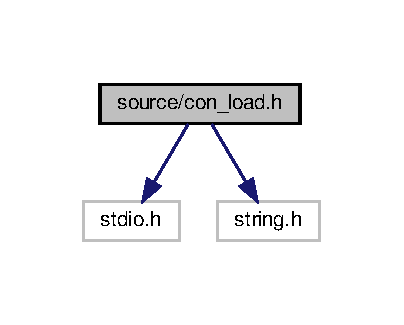
\includegraphics[width=194pt]{con__load_8h__incl}
\end{center}
\end{figure}
This graph shows which files directly or indirectly include this file\+:\nopagebreak
\begin{figure}[H]
\begin{center}
\leavevmode
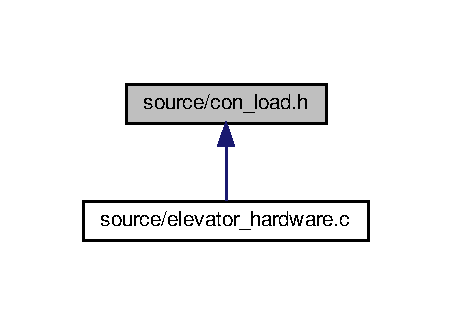
\includegraphics[width=217pt]{con__load_8h__dep__incl}
\end{center}
\end{figure}


\subsection{Detailed Description}
Background file used by \hyperlink{elevator__hardware_8h}{elevator\+\_\+hardware.\+h} to communicate with the elevator. 


\hypertarget{elevator__hardware_8c}{}\section{source/elevator\+\_\+hardware.c File Reference}
\label{elevator__hardware_8c}\index{source/elevator\+\_\+hardware.\+c@{source/elevator\+\_\+hardware.\+c}}


Implementation of the functions in \hyperlink{elevator__hardware_8h}{elevator\+\_\+hardware.\+h}.  


{\ttfamily \#include $<$assert.\+h$>$}\newline
{\ttfamily \#include $<$stdlib.\+h$>$}\newline
{\ttfamily \#include $<$sys/socket.\+h$>$}\newline
{\ttfamily \#include $<$netdb.\+h$>$}\newline
{\ttfamily \#include $<$stdio.\+h$>$}\newline
{\ttfamily \#include $<$pthread.\+h$>$}\newline
{\ttfamily \#include \char`\"{}elevator\+\_\+hardware.\+h\char`\"{}}\newline
{\ttfamily \#include \char`\"{}con\+\_\+load.\+h\char`\"{}}\newline
Include dependency graph for elevator\+\_\+hardware.\+c\+:\nopagebreak
\begin{figure}[H]
\begin{center}
\leavevmode
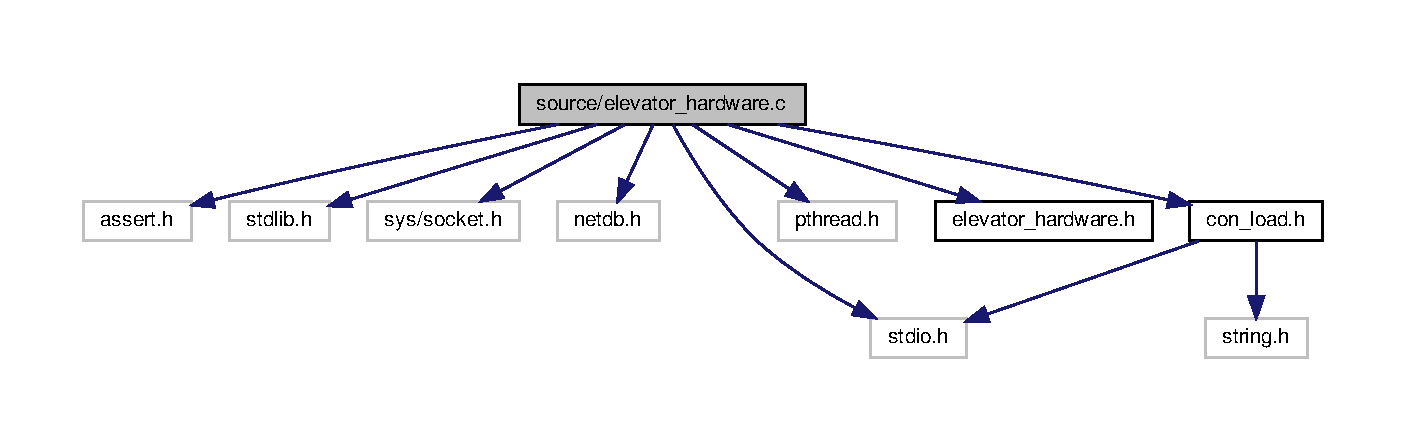
\includegraphics[width=350pt]{elevator__hardware_8c__incl}
\end{center}
\end{figure}
\subsection*{Functions}
\begin{DoxyCompactItemize}
\item 
void \hyperlink{elevator__hardware_8c_a9947d40b2dd08b246692ce64ef60b8c9}{elev\+\_\+init} ()
\item 
void \hyperlink{elevator__hardware_8c_ac7dccb879f6e812e9d245174a0214536}{elev\+\_\+set\+\_\+motor\+\_\+direction} (\hyperlink{elevator__hardware_8h_ac873de158b370a210216e4b4c7fb218f}{elev\+\_\+motor\+\_\+direction\+\_\+t} dirn)
\item 
void \hyperlink{elevator__hardware_8c_a9e81321c63d80ddf1699bc91593cd9d4}{elev\+\_\+set\+\_\+button\+\_\+lamp} (\hyperlink{elevator__hardware_8h_a5457414cc26332731098d18c37a46e6c}{elev\+\_\+button\+\_\+type\+\_\+t} button, int floor, int value)
\item 
void \hyperlink{elevator__hardware_8c_a6af53dd3ebae3a5791ba345eac84d4be}{elev\+\_\+set\+\_\+floor\+\_\+indicator} (int floor)
\item 
void \hyperlink{elevator__hardware_8c_a6ce9a34b8677b483b0d8f9dc47b42c40}{elev\+\_\+set\+\_\+door\+\_\+open\+\_\+lamp} (int value)
\item 
void \hyperlink{elevator__hardware_8c_a85de2a6536b4dd0c83bac19923500740}{elev\+\_\+set\+\_\+stop\+\_\+lamp} (int value)
\item 
int \hyperlink{elevator__hardware_8c_a2350a1635233760719700552a6cb0763}{elev\+\_\+get\+\_\+button\+\_\+signal} (\hyperlink{elevator__hardware_8h_a5457414cc26332731098d18c37a46e6c}{elev\+\_\+button\+\_\+type\+\_\+t} button, int floor)
\item 
int \hyperlink{elevator__hardware_8c_a97d30b7e2538acf5647515638070fdc5}{elev\+\_\+get\+\_\+floor\+\_\+sensor\+\_\+signal} (void)
\item 
int \hyperlink{elevator__hardware_8c_ab702d0ff2d7d03172b7ae3829ba13028}{elev\+\_\+get\+\_\+stop\+\_\+signal} (void)
\item 
int \hyperlink{elevator__hardware_8c_acd97a0fbc9013dc954923e25e90be9df}{elev\+\_\+get\+\_\+obstruction\+\_\+signal} (void)
\end{DoxyCompactItemize}


\subsection{Detailed Description}
Implementation of the functions in \hyperlink{elevator__hardware_8h}{elevator\+\_\+hardware.\+h}. 



\subsection{Function Documentation}
\mbox{\Hypertarget{elevator__hardware_8c_a2350a1635233760719700552a6cb0763}\label{elevator__hardware_8c_a2350a1635233760719700552a6cb0763}} 
\index{elevator\+\_\+hardware.\+c@{elevator\+\_\+hardware.\+c}!elev\+\_\+get\+\_\+button\+\_\+signal@{elev\+\_\+get\+\_\+button\+\_\+signal}}
\index{elev\+\_\+get\+\_\+button\+\_\+signal@{elev\+\_\+get\+\_\+button\+\_\+signal}!elevator\+\_\+hardware.\+c@{elevator\+\_\+hardware.\+c}}
\subsubsection{\texorpdfstring{elev\+\_\+get\+\_\+button\+\_\+signal()}{elev\_get\_button\_signal()}}
{\footnotesize\ttfamily int elev\+\_\+get\+\_\+button\+\_\+signal (\begin{DoxyParamCaption}\item[{\hyperlink{elevator__hardware_8h_a5457414cc26332731098d18c37a46e6c}{elev\+\_\+button\+\_\+type\+\_\+t}}]{button,  }\item[{int}]{floor }\end{DoxyParamCaption})}

Gets a button signal. 
\begin{DoxyParams}[1]{Parameters}
\mbox{\tt in}  & {\em button} & Which button type to check as defined in \hyperlink{elevator__hardware_8h_a5457414cc26332731098d18c37a46e6c}{elev\+\_\+button\+\_\+type\+\_\+t}. \\
\hline
\mbox{\tt in}  & {\em floor} & Which floor to check button. Must be 0-\/3. \\
\hline
\end{DoxyParams}
\begin{DoxyReturn}{Returns}
0 if button is not pushed. 1 if button is pushed. 
\end{DoxyReturn}


Definition at line 96 of file elevator\+\_\+hardware.\+c.

\mbox{\Hypertarget{elevator__hardware_8c_a97d30b7e2538acf5647515638070fdc5}\label{elevator__hardware_8c_a97d30b7e2538acf5647515638070fdc5}} 
\index{elevator\+\_\+hardware.\+c@{elevator\+\_\+hardware.\+c}!elev\+\_\+get\+\_\+floor\+\_\+sensor\+\_\+signal@{elev\+\_\+get\+\_\+floor\+\_\+sensor\+\_\+signal}}
\index{elev\+\_\+get\+\_\+floor\+\_\+sensor\+\_\+signal@{elev\+\_\+get\+\_\+floor\+\_\+sensor\+\_\+signal}!elevator\+\_\+hardware.\+c@{elevator\+\_\+hardware.\+c}}
\subsubsection{\texorpdfstring{elev\+\_\+get\+\_\+floor\+\_\+sensor\+\_\+signal()}{elev\_get\_floor\_sensor\_signal()}}
{\footnotesize\ttfamily int elev\+\_\+get\+\_\+floor\+\_\+sensor\+\_\+signal (\begin{DoxyParamCaption}\item[{void}]{ }\end{DoxyParamCaption})}

Get floor sensor signal. \begin{DoxyReturn}{Returns}
-\/1 if elevator is not on a floor. 0-\/3 if elevator is on floor. 0 is ground floor, 3 is top floor. 
\end{DoxyReturn}


Definition at line 106 of file elevator\+\_\+hardware.\+c.

\mbox{\Hypertarget{elevator__hardware_8c_acd97a0fbc9013dc954923e25e90be9df}\label{elevator__hardware_8c_acd97a0fbc9013dc954923e25e90be9df}} 
\index{elevator\+\_\+hardware.\+c@{elevator\+\_\+hardware.\+c}!elev\+\_\+get\+\_\+obstruction\+\_\+signal@{elev\+\_\+get\+\_\+obstruction\+\_\+signal}}
\index{elev\+\_\+get\+\_\+obstruction\+\_\+signal@{elev\+\_\+get\+\_\+obstruction\+\_\+signal}!elevator\+\_\+hardware.\+c@{elevator\+\_\+hardware.\+c}}
\subsubsection{\texorpdfstring{elev\+\_\+get\+\_\+obstruction\+\_\+signal()}{elev\_get\_obstruction\_signal()}}
{\footnotesize\ttfamily int elev\+\_\+get\+\_\+obstruction\+\_\+signal (\begin{DoxyParamCaption}\item[{void}]{ }\end{DoxyParamCaption})}

Get signal from obstruction switch. \begin{DoxyReturn}{Returns}
1 if obstruction is enabled. 0 if not. 
\end{DoxyReturn}


Definition at line 126 of file elevator\+\_\+hardware.\+c.

\mbox{\Hypertarget{elevator__hardware_8c_ab702d0ff2d7d03172b7ae3829ba13028}\label{elevator__hardware_8c_ab702d0ff2d7d03172b7ae3829ba13028}} 
\index{elevator\+\_\+hardware.\+c@{elevator\+\_\+hardware.\+c}!elev\+\_\+get\+\_\+stop\+\_\+signal@{elev\+\_\+get\+\_\+stop\+\_\+signal}}
\index{elev\+\_\+get\+\_\+stop\+\_\+signal@{elev\+\_\+get\+\_\+stop\+\_\+signal}!elevator\+\_\+hardware.\+c@{elevator\+\_\+hardware.\+c}}
\subsubsection{\texorpdfstring{elev\+\_\+get\+\_\+stop\+\_\+signal()}{elev\_get\_stop\_signal()}}
{\footnotesize\ttfamily int elev\+\_\+get\+\_\+stop\+\_\+signal (\begin{DoxyParamCaption}\item[{void}]{ }\end{DoxyParamCaption})}

Get signal from stop button. \begin{DoxyReturn}{Returns}
1 if stop button is pushed, 0 if not. 
\end{DoxyReturn}


Definition at line 116 of file elevator\+\_\+hardware.\+c.

\mbox{\Hypertarget{elevator__hardware_8c_a9947d40b2dd08b246692ce64ef60b8c9}\label{elevator__hardware_8c_a9947d40b2dd08b246692ce64ef60b8c9}} 
\index{elevator\+\_\+hardware.\+c@{elevator\+\_\+hardware.\+c}!elev\+\_\+init@{elev\+\_\+init}}
\index{elev\+\_\+init@{elev\+\_\+init}!elevator\+\_\+hardware.\+c@{elevator\+\_\+hardware.\+c}}
\subsubsection{\texorpdfstring{elev\+\_\+init()}{elev\_init()}}
{\footnotesize\ttfamily void elev\+\_\+init (\begin{DoxyParamCaption}{ }\end{DoxyParamCaption})}

Initialize elevator. \begin{DoxyReturn}{Returns}
Non-\/zero on success, 0 on failure. 
\end{DoxyReturn}


Definition at line 19 of file elevator\+\_\+hardware.\+c.

\mbox{\Hypertarget{elevator__hardware_8c_a9e81321c63d80ddf1699bc91593cd9d4}\label{elevator__hardware_8c_a9e81321c63d80ddf1699bc91593cd9d4}} 
\index{elevator\+\_\+hardware.\+c@{elevator\+\_\+hardware.\+c}!elev\+\_\+set\+\_\+button\+\_\+lamp@{elev\+\_\+set\+\_\+button\+\_\+lamp}}
\index{elev\+\_\+set\+\_\+button\+\_\+lamp@{elev\+\_\+set\+\_\+button\+\_\+lamp}!elevator\+\_\+hardware.\+c@{elevator\+\_\+hardware.\+c}}
\subsubsection{\texorpdfstring{elev\+\_\+set\+\_\+button\+\_\+lamp()}{elev\_set\_button\_lamp()}}
{\footnotesize\ttfamily void elev\+\_\+set\+\_\+button\+\_\+lamp (\begin{DoxyParamCaption}\item[{\hyperlink{elevator__hardware_8h_a5457414cc26332731098d18c37a46e6c}{elev\+\_\+button\+\_\+type\+\_\+t}}]{button,  }\item[{int}]{floor,  }\item[{int}]{value }\end{DoxyParamCaption})}

Set a button lamp. 
\begin{DoxyParams}[1]{Parameters}
\mbox{\tt in}  & {\em lamp} & Which type of lamp to set as defined in \hyperlink{elevator__hardware_8h_a5457414cc26332731098d18c37a46e6c}{elev\+\_\+button\+\_\+type\+\_\+t}. \\
\hline
\mbox{\tt in}  & {\em floor} & Floor of lamp to set. Must be 0-\/3 \\
\hline
\mbox{\tt in}  & {\em value} & Non-\/zero value turns lamp on, 0 turns lamp off. \\
\hline
\end{DoxyParams}


Definition at line 58 of file elevator\+\_\+hardware.\+c.

Here is the caller graph for this function\+:\nopagebreak
\begin{figure}[H]
\begin{center}
\leavevmode
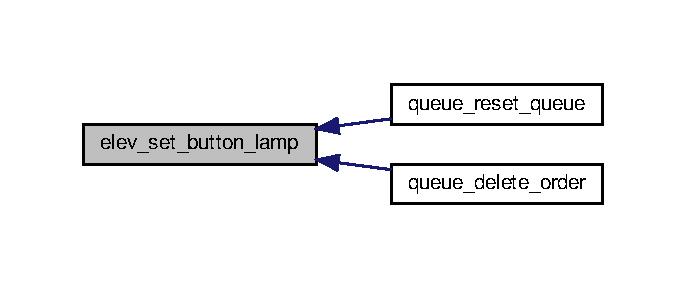
\includegraphics[width=329pt]{elevator__hardware_8c_a9e81321c63d80ddf1699bc91593cd9d4_icgraph}
\end{center}
\end{figure}
\mbox{\Hypertarget{elevator__hardware_8c_a6ce9a34b8677b483b0d8f9dc47b42c40}\label{elevator__hardware_8c_a6ce9a34b8677b483b0d8f9dc47b42c40}} 
\index{elevator\+\_\+hardware.\+c@{elevator\+\_\+hardware.\+c}!elev\+\_\+set\+\_\+door\+\_\+open\+\_\+lamp@{elev\+\_\+set\+\_\+door\+\_\+open\+\_\+lamp}}
\index{elev\+\_\+set\+\_\+door\+\_\+open\+\_\+lamp@{elev\+\_\+set\+\_\+door\+\_\+open\+\_\+lamp}!elevator\+\_\+hardware.\+c@{elevator\+\_\+hardware.\+c}}
\subsubsection{\texorpdfstring{elev\+\_\+set\+\_\+door\+\_\+open\+\_\+lamp()}{elev\_set\_door\_open\_lamp()}}
{\footnotesize\ttfamily void elev\+\_\+set\+\_\+door\+\_\+open\+\_\+lamp (\begin{DoxyParamCaption}\item[{int}]{value }\end{DoxyParamCaption})}

Turn door-\/open lamp on or off. 
\begin{DoxyParams}[1]{Parameters}
\mbox{\tt in}  & {\em value} & Non-\/zero value turns lamp on, 0 turns lamp off. \\
\hline
\end{DoxyParams}


Definition at line 80 of file elevator\+\_\+hardware.\+c.

\mbox{\Hypertarget{elevator__hardware_8c_a6af53dd3ebae3a5791ba345eac84d4be}\label{elevator__hardware_8c_a6af53dd3ebae3a5791ba345eac84d4be}} 
\index{elevator\+\_\+hardware.\+c@{elevator\+\_\+hardware.\+c}!elev\+\_\+set\+\_\+floor\+\_\+indicator@{elev\+\_\+set\+\_\+floor\+\_\+indicator}}
\index{elev\+\_\+set\+\_\+floor\+\_\+indicator@{elev\+\_\+set\+\_\+floor\+\_\+indicator}!elevator\+\_\+hardware.\+c@{elevator\+\_\+hardware.\+c}}
\subsubsection{\texorpdfstring{elev\+\_\+set\+\_\+floor\+\_\+indicator()}{elev\_set\_floor\_indicator()}}
{\footnotesize\ttfamily void elev\+\_\+set\+\_\+floor\+\_\+indicator (\begin{DoxyParamCaption}\item[{int}]{floor }\end{DoxyParamCaption})}

Set floor indicator lamp for a given floor. 
\begin{DoxyParams}[1]{Parameters}
\mbox{\tt in}  & {\em floor} & Which floor lamp to turn on. Other floor lamps are turned off. \\
\hline
\end{DoxyParams}


Definition at line 70 of file elevator\+\_\+hardware.\+c.

\mbox{\Hypertarget{elevator__hardware_8c_ac7dccb879f6e812e9d245174a0214536}\label{elevator__hardware_8c_ac7dccb879f6e812e9d245174a0214536}} 
\index{elevator\+\_\+hardware.\+c@{elevator\+\_\+hardware.\+c}!elev\+\_\+set\+\_\+motor\+\_\+direction@{elev\+\_\+set\+\_\+motor\+\_\+direction}}
\index{elev\+\_\+set\+\_\+motor\+\_\+direction@{elev\+\_\+set\+\_\+motor\+\_\+direction}!elevator\+\_\+hardware.\+c@{elevator\+\_\+hardware.\+c}}
\subsubsection{\texorpdfstring{elev\+\_\+set\+\_\+motor\+\_\+direction()}{elev\_set\_motor\_direction()}}
{\footnotesize\ttfamily void elev\+\_\+set\+\_\+motor\+\_\+direction (\begin{DoxyParamCaption}\item[{\hyperlink{elevator__hardware_8h_ac873de158b370a210216e4b4c7fb218f}{elev\+\_\+motor\+\_\+direction\+\_\+t}}]{dirn }\end{DoxyParamCaption})}

Sets the motor direction of the elevator. 
\begin{DoxyParams}[1]{Parameters}
\mbox{\tt in}  & {\em dirn} & New direction of the elevator. \\
\hline
\end{DoxyParams}


Definition at line 51 of file elevator\+\_\+hardware.\+c.

\mbox{\Hypertarget{elevator__hardware_8c_a85de2a6536b4dd0c83bac19923500740}\label{elevator__hardware_8c_a85de2a6536b4dd0c83bac19923500740}} 
\index{elevator\+\_\+hardware.\+c@{elevator\+\_\+hardware.\+c}!elev\+\_\+set\+\_\+stop\+\_\+lamp@{elev\+\_\+set\+\_\+stop\+\_\+lamp}}
\index{elev\+\_\+set\+\_\+stop\+\_\+lamp@{elev\+\_\+set\+\_\+stop\+\_\+lamp}!elevator\+\_\+hardware.\+c@{elevator\+\_\+hardware.\+c}}
\subsubsection{\texorpdfstring{elev\+\_\+set\+\_\+stop\+\_\+lamp()}{elev\_set\_stop\_lamp()}}
{\footnotesize\ttfamily void elev\+\_\+set\+\_\+stop\+\_\+lamp (\begin{DoxyParamCaption}\item[{int}]{value }\end{DoxyParamCaption})}

Turn stop lamp on or off. 
\begin{DoxyParams}[1]{Parameters}
\mbox{\tt in}  & {\em value} & Non-\/zero value turns lamp on, 0 turns lamp off. \\
\hline
\end{DoxyParams}


Definition at line 87 of file elevator\+\_\+hardware.\+c.


\hypertarget{elevator__hardware_8h}{}\section{source/elevator\+\_\+hardware.h File Reference}
\label{elevator__hardware_8h}\index{source/elevator\+\_\+hardware.\+h@{source/elevator\+\_\+hardware.\+h}}


The driver that communicates with the elevator hardware. This is done through a server that is set up on a port on the machine and communicates with the elevator hardware. The function interactions are identical to the driver provided by the lab instructor in the Embedded Systems course.  


This graph shows which files directly or indirectly include this file\+:\nopagebreak
\begin{figure}[H]
\begin{center}
\leavevmode
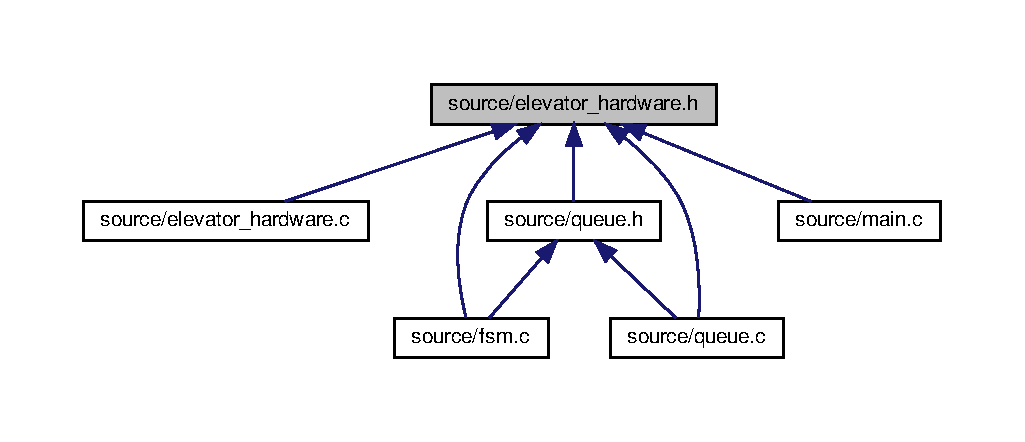
\includegraphics[width=350pt]{elevator__hardware_8h__dep__incl}
\end{center}
\end{figure}
\subsection*{Macros}
\begin{DoxyCompactItemize}
\item 
\mbox{\Hypertarget{elevator__hardware_8h_ae0592e3739e5e1e76234bb1caf9d1305}\label{elevator__hardware_8h_ae0592e3739e5e1e76234bb1caf9d1305}} 
\#define \hyperlink{elevator__hardware_8h_ae0592e3739e5e1e76234bb1caf9d1305}{N\+\_\+\+F\+L\+O\+O\+RS}~4
\begin{DoxyCompactList}\small\item\em Number of floors in \hyperlink{fsm_8h_a5b3a976f46b9e6993f1692a09bf2fd60}{floor\+\_\+t} without O\+R\+D\+E\+R\+\_\+\+F\+L\+O\+O\+R\+\_\+\+U\+N\+K\+N\+O\+WN, also Hardware-\/dependent. \end{DoxyCompactList}\item 
\mbox{\Hypertarget{elevator__hardware_8h_a271dda243b0f5bd7d2053d258eb71962}\label{elevator__hardware_8h_a271dda243b0f5bd7d2053d258eb71962}} 
\#define \hyperlink{elevator__hardware_8h_a271dda243b0f5bd7d2053d258eb71962}{N\+\_\+\+B\+U\+T\+T\+O\+NS}~3
\begin{DoxyCompactList}\small\item\em Number of button types in \hyperlink{elevator__hardware_8h_a5457414cc26332731098d18c37a46e6c}{elev\+\_\+button\+\_\+type\+\_\+t}. \end{DoxyCompactList}\end{DoxyCompactItemize}
\subsection*{Enumerations}
\begin{DoxyCompactItemize}
\item 
enum \hyperlink{elevator__hardware_8h_ac873de158b370a210216e4b4c7fb218f}{elev\+\_\+motor\+\_\+direction\+\_\+t} \{ \hyperlink{elevator__hardware_8h_ac873de158b370a210216e4b4c7fb218fa3164bca805ecbf4446a19625a7b55411}{D\+I\+R\+N\+\_\+\+D\+O\+WN} = -\/1, 
\hyperlink{elevator__hardware_8h_ac873de158b370a210216e4b4c7fb218fa72dbefe6c155fb5ea5c8d242a8079646}{D\+I\+R\+N\+\_\+\+S\+T\+OP} = 0, 
\hyperlink{elevator__hardware_8h_ac873de158b370a210216e4b4c7fb218fa92f9028d3af929e10b735b77e0c8de60}{D\+I\+R\+N\+\_\+\+UP} = 1
 \}
\item 
enum \hyperlink{elevator__hardware_8h_a5457414cc26332731098d18c37a46e6c}{elev\+\_\+button\+\_\+type\+\_\+t} \{ \hyperlink{elevator__hardware_8h_a5457414cc26332731098d18c37a46e6ca3e1ab9a7c324a535e118f45c1eec8067}{B\+U\+T\+T\+O\+N\+\_\+\+C\+A\+L\+L\+\_\+\+UP} = 0, 
\hyperlink{elevator__hardware_8h_a5457414cc26332731098d18c37a46e6ca740c1be4edf3a5b2849e06704ad8e12f}{B\+U\+T\+T\+O\+N\+\_\+\+C\+A\+L\+L\+\_\+\+D\+O\+WN} = 1, 
\hyperlink{elevator__hardware_8h_a5457414cc26332731098d18c37a46e6cad20de8df1af7d13ad4e904f918dc09d1}{B\+U\+T\+T\+O\+N\+\_\+\+C\+O\+M\+M\+A\+ND} = 2
 \}
\end{DoxyCompactItemize}
\subsection*{Functions}
\begin{DoxyCompactItemize}
\item 
void \hyperlink{elevator__hardware_8h_a9947d40b2dd08b246692ce64ef60b8c9}{elev\+\_\+init} ()
\item 
void \hyperlink{elevator__hardware_8h_ac7dccb879f6e812e9d245174a0214536}{elev\+\_\+set\+\_\+motor\+\_\+direction} (\hyperlink{elevator__hardware_8h_ac873de158b370a210216e4b4c7fb218f}{elev\+\_\+motor\+\_\+direction\+\_\+t} dirn)
\item 
void \hyperlink{elevator__hardware_8h_a9e81321c63d80ddf1699bc91593cd9d4}{elev\+\_\+set\+\_\+button\+\_\+lamp} (\hyperlink{elevator__hardware_8h_a5457414cc26332731098d18c37a46e6c}{elev\+\_\+button\+\_\+type\+\_\+t} button, int floor, int value)
\item 
void \hyperlink{elevator__hardware_8h_a6af53dd3ebae3a5791ba345eac84d4be}{elev\+\_\+set\+\_\+floor\+\_\+indicator} (int floor)
\item 
void \hyperlink{elevator__hardware_8h_a6ce9a34b8677b483b0d8f9dc47b42c40}{elev\+\_\+set\+\_\+door\+\_\+open\+\_\+lamp} (int value)
\item 
void \hyperlink{elevator__hardware_8h_a85de2a6536b4dd0c83bac19923500740}{elev\+\_\+set\+\_\+stop\+\_\+lamp} (int value)
\item 
int \hyperlink{elevator__hardware_8h_a2350a1635233760719700552a6cb0763}{elev\+\_\+get\+\_\+button\+\_\+signal} (\hyperlink{elevator__hardware_8h_a5457414cc26332731098d18c37a46e6c}{elev\+\_\+button\+\_\+type\+\_\+t} button, int floor)
\item 
int \hyperlink{elevator__hardware_8h_a97d30b7e2538acf5647515638070fdc5}{elev\+\_\+get\+\_\+floor\+\_\+sensor\+\_\+signal} (void)
\item 
int \hyperlink{elevator__hardware_8h_ab702d0ff2d7d03172b7ae3829ba13028}{elev\+\_\+get\+\_\+stop\+\_\+signal} (void)
\item 
int \hyperlink{elevator__hardware_8h_acd97a0fbc9013dc954923e25e90be9df}{elev\+\_\+get\+\_\+obstruction\+\_\+signal} (void)
\end{DoxyCompactItemize}


\subsection{Detailed Description}
The driver that communicates with the elevator hardware. This is done through a server that is set up on a port on the machine and communicates with the elevator hardware. The function interactions are identical to the driver provided by the lab instructor in the Embedded Systems course. 



\subsection{Enumeration Type Documentation}
\mbox{\Hypertarget{elevator__hardware_8h_a5457414cc26332731098d18c37a46e6c}\label{elevator__hardware_8h_a5457414cc26332731098d18c37a46e6c}} 
\index{elevator\+\_\+hardware.\+h@{elevator\+\_\+hardware.\+h}!elev\+\_\+button\+\_\+type\+\_\+t@{elev\+\_\+button\+\_\+type\+\_\+t}}
\index{elev\+\_\+button\+\_\+type\+\_\+t@{elev\+\_\+button\+\_\+type\+\_\+t}!elevator\+\_\+hardware.\+h@{elevator\+\_\+hardware.\+h}}
\subsubsection{\texorpdfstring{elev\+\_\+button\+\_\+type\+\_\+t}{elev\_button\_type\_t}}
{\footnotesize\ttfamily enum \hyperlink{elevator__hardware_8h_a5457414cc26332731098d18c37a46e6c}{elev\+\_\+button\+\_\+type\+\_\+t}}

Button types for function \hyperlink{elevator__hardware_8h_a9e81321c63d80ddf1699bc91593cd9d4}{elev\+\_\+set\+\_\+button\+\_\+lamp()} and elev\+\_\+get\+\_\+button(). \begin{DoxyEnumFields}{Enumerator}
\raisebox{\heightof{T}}[0pt][0pt]{\index{B\+U\+T\+T\+O\+N\+\_\+\+C\+A\+L\+L\+\_\+\+UP@{B\+U\+T\+T\+O\+N\+\_\+\+C\+A\+L\+L\+\_\+\+UP}!elevator\+\_\+hardware.\+h@{elevator\+\_\+hardware.\+h}}\index{elevator\+\_\+hardware.\+h@{elevator\+\_\+hardware.\+h}!B\+U\+T\+T\+O\+N\+\_\+\+C\+A\+L\+L\+\_\+\+UP@{B\+U\+T\+T\+O\+N\+\_\+\+C\+A\+L\+L\+\_\+\+UP}}}\mbox{\Hypertarget{elevator__hardware_8h_a5457414cc26332731098d18c37a46e6ca3e1ab9a7c324a535e118f45c1eec8067}\label{elevator__hardware_8h_a5457414cc26332731098d18c37a46e6ca3e1ab9a7c324a535e118f45c1eec8067}} 
B\+U\+T\+T\+O\+N\+\_\+\+C\+A\+L\+L\+\_\+\+UP&Elevator hall order in upwards direction. \\
\hline

\raisebox{\heightof{T}}[0pt][0pt]{\index{B\+U\+T\+T\+O\+N\+\_\+\+C\+A\+L\+L\+\_\+\+D\+O\+WN@{B\+U\+T\+T\+O\+N\+\_\+\+C\+A\+L\+L\+\_\+\+D\+O\+WN}!elevator\+\_\+hardware.\+h@{elevator\+\_\+hardware.\+h}}\index{elevator\+\_\+hardware.\+h@{elevator\+\_\+hardware.\+h}!B\+U\+T\+T\+O\+N\+\_\+\+C\+A\+L\+L\+\_\+\+D\+O\+WN@{B\+U\+T\+T\+O\+N\+\_\+\+C\+A\+L\+L\+\_\+\+D\+O\+WN}}}\mbox{\Hypertarget{elevator__hardware_8h_a5457414cc26332731098d18c37a46e6ca740c1be4edf3a5b2849e06704ad8e12f}\label{elevator__hardware_8h_a5457414cc26332731098d18c37a46e6ca740c1be4edf3a5b2849e06704ad8e12f}} 
B\+U\+T\+T\+O\+N\+\_\+\+C\+A\+L\+L\+\_\+\+D\+O\+WN&Elevator hall order in downwards direction. \\
\hline

\raisebox{\heightof{T}}[0pt][0pt]{\index{B\+U\+T\+T\+O\+N\+\_\+\+C\+O\+M\+M\+A\+ND@{B\+U\+T\+T\+O\+N\+\_\+\+C\+O\+M\+M\+A\+ND}!elevator\+\_\+hardware.\+h@{elevator\+\_\+hardware.\+h}}\index{elevator\+\_\+hardware.\+h@{elevator\+\_\+hardware.\+h}!B\+U\+T\+T\+O\+N\+\_\+\+C\+O\+M\+M\+A\+ND@{B\+U\+T\+T\+O\+N\+\_\+\+C\+O\+M\+M\+A\+ND}}}\mbox{\Hypertarget{elevator__hardware_8h_a5457414cc26332731098d18c37a46e6cad20de8df1af7d13ad4e904f918dc09d1}\label{elevator__hardware_8h_a5457414cc26332731098d18c37a46e6cad20de8df1af7d13ad4e904f918dc09d1}} 
B\+U\+T\+T\+O\+N\+\_\+\+C\+O\+M\+M\+A\+ND&Elevator cab order from within the elevator. \\
\hline

\end{DoxyEnumFields}


Definition at line 30 of file elevator\+\_\+hardware.\+h.

\mbox{\Hypertarget{elevator__hardware_8h_ac873de158b370a210216e4b4c7fb218f}\label{elevator__hardware_8h_ac873de158b370a210216e4b4c7fb218f}} 
\index{elevator\+\_\+hardware.\+h@{elevator\+\_\+hardware.\+h}!elev\+\_\+motor\+\_\+direction\+\_\+t@{elev\+\_\+motor\+\_\+direction\+\_\+t}}
\index{elev\+\_\+motor\+\_\+direction\+\_\+t@{elev\+\_\+motor\+\_\+direction\+\_\+t}!elevator\+\_\+hardware.\+h@{elevator\+\_\+hardware.\+h}}
\subsubsection{\texorpdfstring{elev\+\_\+motor\+\_\+direction\+\_\+t}{elev\_motor\_direction\_t}}
{\footnotesize\ttfamily enum \hyperlink{elevator__hardware_8h_ac873de158b370a210216e4b4c7fb218f}{elev\+\_\+motor\+\_\+direction\+\_\+t}}

Motor direction for function \hyperlink{elevator__hardware_8h_ac7dccb879f6e812e9d245174a0214536}{elev\+\_\+set\+\_\+motor\+\_\+direction()}. \begin{DoxyEnumFields}{Enumerator}
\raisebox{\heightof{T}}[0pt][0pt]{\index{D\+I\+R\+N\+\_\+\+D\+O\+WN@{D\+I\+R\+N\+\_\+\+D\+O\+WN}!elevator\+\_\+hardware.\+h@{elevator\+\_\+hardware.\+h}}\index{elevator\+\_\+hardware.\+h@{elevator\+\_\+hardware.\+h}!D\+I\+R\+N\+\_\+\+D\+O\+WN@{D\+I\+R\+N\+\_\+\+D\+O\+WN}}}\mbox{\Hypertarget{elevator__hardware_8h_ac873de158b370a210216e4b4c7fb218fa3164bca805ecbf4446a19625a7b55411}\label{elevator__hardware_8h_ac873de158b370a210216e4b4c7fb218fa3164bca805ecbf4446a19625a7b55411}} 
D\+I\+R\+N\+\_\+\+D\+O\+WN&Elevator motor direction downwards. \\
\hline

\raisebox{\heightof{T}}[0pt][0pt]{\index{D\+I\+R\+N\+\_\+\+S\+T\+OP@{D\+I\+R\+N\+\_\+\+S\+T\+OP}!elevator\+\_\+hardware.\+h@{elevator\+\_\+hardware.\+h}}\index{elevator\+\_\+hardware.\+h@{elevator\+\_\+hardware.\+h}!D\+I\+R\+N\+\_\+\+S\+T\+OP@{D\+I\+R\+N\+\_\+\+S\+T\+OP}}}\mbox{\Hypertarget{elevator__hardware_8h_ac873de158b370a210216e4b4c7fb218fa72dbefe6c155fb5ea5c8d242a8079646}\label{elevator__hardware_8h_ac873de158b370a210216e4b4c7fb218fa72dbefe6c155fb5ea5c8d242a8079646}} 
D\+I\+R\+N\+\_\+\+S\+T\+OP&Elevator motor stopped. \\
\hline

\raisebox{\heightof{T}}[0pt][0pt]{\index{D\+I\+R\+N\+\_\+\+UP@{D\+I\+R\+N\+\_\+\+UP}!elevator\+\_\+hardware.\+h@{elevator\+\_\+hardware.\+h}}\index{elevator\+\_\+hardware.\+h@{elevator\+\_\+hardware.\+h}!D\+I\+R\+N\+\_\+\+UP@{D\+I\+R\+N\+\_\+\+UP}}}\mbox{\Hypertarget{elevator__hardware_8h_ac873de158b370a210216e4b4c7fb218fa92f9028d3af929e10b735b77e0c8de60}\label{elevator__hardware_8h_ac873de158b370a210216e4b4c7fb218fa92f9028d3af929e10b735b77e0c8de60}} 
D\+I\+R\+N\+\_\+\+UP&Elevator motor direction upwards. \\
\hline

\end{DoxyEnumFields}


Definition at line 21 of file elevator\+\_\+hardware.\+h.



\subsection{Function Documentation}
\mbox{\Hypertarget{elevator__hardware_8h_a2350a1635233760719700552a6cb0763}\label{elevator__hardware_8h_a2350a1635233760719700552a6cb0763}} 
\index{elevator\+\_\+hardware.\+h@{elevator\+\_\+hardware.\+h}!elev\+\_\+get\+\_\+button\+\_\+signal@{elev\+\_\+get\+\_\+button\+\_\+signal}}
\index{elev\+\_\+get\+\_\+button\+\_\+signal@{elev\+\_\+get\+\_\+button\+\_\+signal}!elevator\+\_\+hardware.\+h@{elevator\+\_\+hardware.\+h}}
\subsubsection{\texorpdfstring{elev\+\_\+get\+\_\+button\+\_\+signal()}{elev\_get\_button\_signal()}}
{\footnotesize\ttfamily int elev\+\_\+get\+\_\+button\+\_\+signal (\begin{DoxyParamCaption}\item[{\hyperlink{elevator__hardware_8h_a5457414cc26332731098d18c37a46e6c}{elev\+\_\+button\+\_\+type\+\_\+t}}]{button,  }\item[{int}]{floor }\end{DoxyParamCaption})}

Gets a button signal. 
\begin{DoxyParams}[1]{Parameters}
\mbox{\tt in}  & {\em button} & Which button type to check as defined in \hyperlink{elevator__hardware_8h_a5457414cc26332731098d18c37a46e6c}{elev\+\_\+button\+\_\+type\+\_\+t}. \\
\hline
\mbox{\tt in}  & {\em floor} & Which floor to check button. Must be 0-\/3. \\
\hline
\end{DoxyParams}
\begin{DoxyReturn}{Returns}
0 if button is not pushed. 1 if button is pushed. 
\end{DoxyReturn}


Definition at line 96 of file elevator\+\_\+hardware.\+c.

\mbox{\Hypertarget{elevator__hardware_8h_a97d30b7e2538acf5647515638070fdc5}\label{elevator__hardware_8h_a97d30b7e2538acf5647515638070fdc5}} 
\index{elevator\+\_\+hardware.\+h@{elevator\+\_\+hardware.\+h}!elev\+\_\+get\+\_\+floor\+\_\+sensor\+\_\+signal@{elev\+\_\+get\+\_\+floor\+\_\+sensor\+\_\+signal}}
\index{elev\+\_\+get\+\_\+floor\+\_\+sensor\+\_\+signal@{elev\+\_\+get\+\_\+floor\+\_\+sensor\+\_\+signal}!elevator\+\_\+hardware.\+h@{elevator\+\_\+hardware.\+h}}
\subsubsection{\texorpdfstring{elev\+\_\+get\+\_\+floor\+\_\+sensor\+\_\+signal()}{elev\_get\_floor\_sensor\_signal()}}
{\footnotesize\ttfamily int elev\+\_\+get\+\_\+floor\+\_\+sensor\+\_\+signal (\begin{DoxyParamCaption}\item[{void}]{ }\end{DoxyParamCaption})}

Get floor sensor signal. \begin{DoxyReturn}{Returns}
-\/1 if elevator is not on a floor. 0-\/3 if elevator is on floor. 0 is ground floor, 3 is top floor. 
\end{DoxyReturn}


Definition at line 106 of file elevator\+\_\+hardware.\+c.

\mbox{\Hypertarget{elevator__hardware_8h_acd97a0fbc9013dc954923e25e90be9df}\label{elevator__hardware_8h_acd97a0fbc9013dc954923e25e90be9df}} 
\index{elevator\+\_\+hardware.\+h@{elevator\+\_\+hardware.\+h}!elev\+\_\+get\+\_\+obstruction\+\_\+signal@{elev\+\_\+get\+\_\+obstruction\+\_\+signal}}
\index{elev\+\_\+get\+\_\+obstruction\+\_\+signal@{elev\+\_\+get\+\_\+obstruction\+\_\+signal}!elevator\+\_\+hardware.\+h@{elevator\+\_\+hardware.\+h}}
\subsubsection{\texorpdfstring{elev\+\_\+get\+\_\+obstruction\+\_\+signal()}{elev\_get\_obstruction\_signal()}}
{\footnotesize\ttfamily int elev\+\_\+get\+\_\+obstruction\+\_\+signal (\begin{DoxyParamCaption}\item[{void}]{ }\end{DoxyParamCaption})}

Get signal from obstruction switch. \begin{DoxyReturn}{Returns}
1 if obstruction is enabled. 0 if not. 
\end{DoxyReturn}


Definition at line 126 of file elevator\+\_\+hardware.\+c.

\mbox{\Hypertarget{elevator__hardware_8h_ab702d0ff2d7d03172b7ae3829ba13028}\label{elevator__hardware_8h_ab702d0ff2d7d03172b7ae3829ba13028}} 
\index{elevator\+\_\+hardware.\+h@{elevator\+\_\+hardware.\+h}!elev\+\_\+get\+\_\+stop\+\_\+signal@{elev\+\_\+get\+\_\+stop\+\_\+signal}}
\index{elev\+\_\+get\+\_\+stop\+\_\+signal@{elev\+\_\+get\+\_\+stop\+\_\+signal}!elevator\+\_\+hardware.\+h@{elevator\+\_\+hardware.\+h}}
\subsubsection{\texorpdfstring{elev\+\_\+get\+\_\+stop\+\_\+signal()}{elev\_get\_stop\_signal()}}
{\footnotesize\ttfamily int elev\+\_\+get\+\_\+stop\+\_\+signal (\begin{DoxyParamCaption}\item[{void}]{ }\end{DoxyParamCaption})}

Get signal from stop button. \begin{DoxyReturn}{Returns}
1 if stop button is pushed, 0 if not. 
\end{DoxyReturn}


Definition at line 116 of file elevator\+\_\+hardware.\+c.

\mbox{\Hypertarget{elevator__hardware_8h_a9947d40b2dd08b246692ce64ef60b8c9}\label{elevator__hardware_8h_a9947d40b2dd08b246692ce64ef60b8c9}} 
\index{elevator\+\_\+hardware.\+h@{elevator\+\_\+hardware.\+h}!elev\+\_\+init@{elev\+\_\+init}}
\index{elev\+\_\+init@{elev\+\_\+init}!elevator\+\_\+hardware.\+h@{elevator\+\_\+hardware.\+h}}
\subsubsection{\texorpdfstring{elev\+\_\+init()}{elev\_init()}}
{\footnotesize\ttfamily void elev\+\_\+init (\begin{DoxyParamCaption}{ }\end{DoxyParamCaption})}

Initialize elevator. \begin{DoxyReturn}{Returns}
Non-\/zero on success, 0 on failure. 
\end{DoxyReturn}


Definition at line 19 of file elevator\+\_\+hardware.\+c.

\mbox{\Hypertarget{elevator__hardware_8h_a9e81321c63d80ddf1699bc91593cd9d4}\label{elevator__hardware_8h_a9e81321c63d80ddf1699bc91593cd9d4}} 
\index{elevator\+\_\+hardware.\+h@{elevator\+\_\+hardware.\+h}!elev\+\_\+set\+\_\+button\+\_\+lamp@{elev\+\_\+set\+\_\+button\+\_\+lamp}}
\index{elev\+\_\+set\+\_\+button\+\_\+lamp@{elev\+\_\+set\+\_\+button\+\_\+lamp}!elevator\+\_\+hardware.\+h@{elevator\+\_\+hardware.\+h}}
\subsubsection{\texorpdfstring{elev\+\_\+set\+\_\+button\+\_\+lamp()}{elev\_set\_button\_lamp()}}
{\footnotesize\ttfamily void elev\+\_\+set\+\_\+button\+\_\+lamp (\begin{DoxyParamCaption}\item[{\hyperlink{elevator__hardware_8h_a5457414cc26332731098d18c37a46e6c}{elev\+\_\+button\+\_\+type\+\_\+t}}]{button,  }\item[{int}]{floor,  }\item[{int}]{value }\end{DoxyParamCaption})}

Set a button lamp. 
\begin{DoxyParams}[1]{Parameters}
\mbox{\tt in}  & {\em lamp} & Which type of lamp to set as defined in \hyperlink{elevator__hardware_8h_a5457414cc26332731098d18c37a46e6c}{elev\+\_\+button\+\_\+type\+\_\+t}. \\
\hline
\mbox{\tt in}  & {\em floor} & Floor of lamp to set. Must be 0-\/3 \\
\hline
\mbox{\tt in}  & {\em value} & Non-\/zero value turns lamp on, 0 turns lamp off. \\
\hline
\end{DoxyParams}


Definition at line 58 of file elevator\+\_\+hardware.\+c.

Here is the caller graph for this function\+:\nopagebreak
\begin{figure}[H]
\begin{center}
\leavevmode
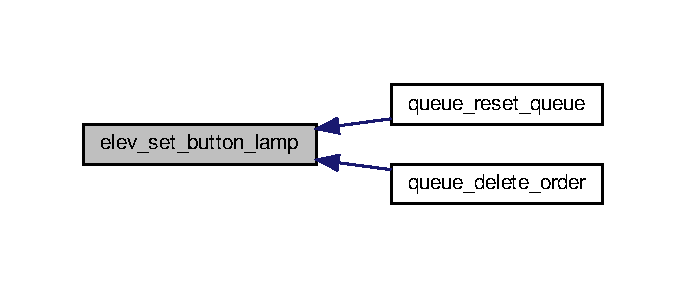
\includegraphics[width=329pt]{elevator__hardware_8h_a9e81321c63d80ddf1699bc91593cd9d4_icgraph}
\end{center}
\end{figure}
\mbox{\Hypertarget{elevator__hardware_8h_a6ce9a34b8677b483b0d8f9dc47b42c40}\label{elevator__hardware_8h_a6ce9a34b8677b483b0d8f9dc47b42c40}} 
\index{elevator\+\_\+hardware.\+h@{elevator\+\_\+hardware.\+h}!elev\+\_\+set\+\_\+door\+\_\+open\+\_\+lamp@{elev\+\_\+set\+\_\+door\+\_\+open\+\_\+lamp}}
\index{elev\+\_\+set\+\_\+door\+\_\+open\+\_\+lamp@{elev\+\_\+set\+\_\+door\+\_\+open\+\_\+lamp}!elevator\+\_\+hardware.\+h@{elevator\+\_\+hardware.\+h}}
\subsubsection{\texorpdfstring{elev\+\_\+set\+\_\+door\+\_\+open\+\_\+lamp()}{elev\_set\_door\_open\_lamp()}}
{\footnotesize\ttfamily void elev\+\_\+set\+\_\+door\+\_\+open\+\_\+lamp (\begin{DoxyParamCaption}\item[{int}]{value }\end{DoxyParamCaption})}

Turn door-\/open lamp on or off. 
\begin{DoxyParams}[1]{Parameters}
\mbox{\tt in}  & {\em value} & Non-\/zero value turns lamp on, 0 turns lamp off. \\
\hline
\end{DoxyParams}


Definition at line 80 of file elevator\+\_\+hardware.\+c.

\mbox{\Hypertarget{elevator__hardware_8h_a6af53dd3ebae3a5791ba345eac84d4be}\label{elevator__hardware_8h_a6af53dd3ebae3a5791ba345eac84d4be}} 
\index{elevator\+\_\+hardware.\+h@{elevator\+\_\+hardware.\+h}!elev\+\_\+set\+\_\+floor\+\_\+indicator@{elev\+\_\+set\+\_\+floor\+\_\+indicator}}
\index{elev\+\_\+set\+\_\+floor\+\_\+indicator@{elev\+\_\+set\+\_\+floor\+\_\+indicator}!elevator\+\_\+hardware.\+h@{elevator\+\_\+hardware.\+h}}
\subsubsection{\texorpdfstring{elev\+\_\+set\+\_\+floor\+\_\+indicator()}{elev\_set\_floor\_indicator()}}
{\footnotesize\ttfamily void elev\+\_\+set\+\_\+floor\+\_\+indicator (\begin{DoxyParamCaption}\item[{int}]{floor }\end{DoxyParamCaption})}

Set floor indicator lamp for a given floor. 
\begin{DoxyParams}[1]{Parameters}
\mbox{\tt in}  & {\em floor} & Which floor lamp to turn on. Other floor lamps are turned off. \\
\hline
\end{DoxyParams}


Definition at line 70 of file elevator\+\_\+hardware.\+c.

\mbox{\Hypertarget{elevator__hardware_8h_ac7dccb879f6e812e9d245174a0214536}\label{elevator__hardware_8h_ac7dccb879f6e812e9d245174a0214536}} 
\index{elevator\+\_\+hardware.\+h@{elevator\+\_\+hardware.\+h}!elev\+\_\+set\+\_\+motor\+\_\+direction@{elev\+\_\+set\+\_\+motor\+\_\+direction}}
\index{elev\+\_\+set\+\_\+motor\+\_\+direction@{elev\+\_\+set\+\_\+motor\+\_\+direction}!elevator\+\_\+hardware.\+h@{elevator\+\_\+hardware.\+h}}
\subsubsection{\texorpdfstring{elev\+\_\+set\+\_\+motor\+\_\+direction()}{elev\_set\_motor\_direction()}}
{\footnotesize\ttfamily void elev\+\_\+set\+\_\+motor\+\_\+direction (\begin{DoxyParamCaption}\item[{\hyperlink{elevator__hardware_8h_ac873de158b370a210216e4b4c7fb218f}{elev\+\_\+motor\+\_\+direction\+\_\+t}}]{dirn }\end{DoxyParamCaption})}

Sets the motor direction of the elevator. 
\begin{DoxyParams}[1]{Parameters}
\mbox{\tt in}  & {\em dirn} & New direction of the elevator. \\
\hline
\end{DoxyParams}


Definition at line 51 of file elevator\+\_\+hardware.\+c.

\mbox{\Hypertarget{elevator__hardware_8h_a85de2a6536b4dd0c83bac19923500740}\label{elevator__hardware_8h_a85de2a6536b4dd0c83bac19923500740}} 
\index{elevator\+\_\+hardware.\+h@{elevator\+\_\+hardware.\+h}!elev\+\_\+set\+\_\+stop\+\_\+lamp@{elev\+\_\+set\+\_\+stop\+\_\+lamp}}
\index{elev\+\_\+set\+\_\+stop\+\_\+lamp@{elev\+\_\+set\+\_\+stop\+\_\+lamp}!elevator\+\_\+hardware.\+h@{elevator\+\_\+hardware.\+h}}
\subsubsection{\texorpdfstring{elev\+\_\+set\+\_\+stop\+\_\+lamp()}{elev\_set\_stop\_lamp()}}
{\footnotesize\ttfamily void elev\+\_\+set\+\_\+stop\+\_\+lamp (\begin{DoxyParamCaption}\item[{int}]{value }\end{DoxyParamCaption})}

Turn stop lamp on or off. 
\begin{DoxyParams}[1]{Parameters}
\mbox{\tt in}  & {\em value} & Non-\/zero value turns lamp on, 0 turns lamp off. \\
\hline
\end{DoxyParams}


Definition at line 87 of file elevator\+\_\+hardware.\+c.


\hypertarget{fsm_8c}{}\section{source/fsm.c File Reference}
\label{fsm_8c}\index{source/fsm.\+c@{source/fsm.\+c}}


Implementation of the functions in \hyperlink{fsm_8h}{fsm.\+h}.  


{\ttfamily \#include $<$stdio.\+h$>$}\newline
{\ttfamily \#include $<$stdint.\+h$>$}\newline
{\ttfamily \#include $<$unistd.\+h$>$}\newline
{\ttfamily \#include $<$time.\+h$>$}\newline
{\ttfamily \#include $<$assert.\+h$>$}\newline
{\ttfamily \#include \char`\"{}elevator\+\_\+hardware.\+h\char`\"{}}\newline
{\ttfamily \#include \char`\"{}fsm.\+h\char`\"{}}\newline
{\ttfamily \#include \char`\"{}queue.\+h\char`\"{}}\newline
{\ttfamily \#include \char`\"{}timer.\+h\char`\"{}}\newline
Include dependency graph for fsm.\+c\+:\nopagebreak
\begin{figure}[H]
\begin{center}
\leavevmode
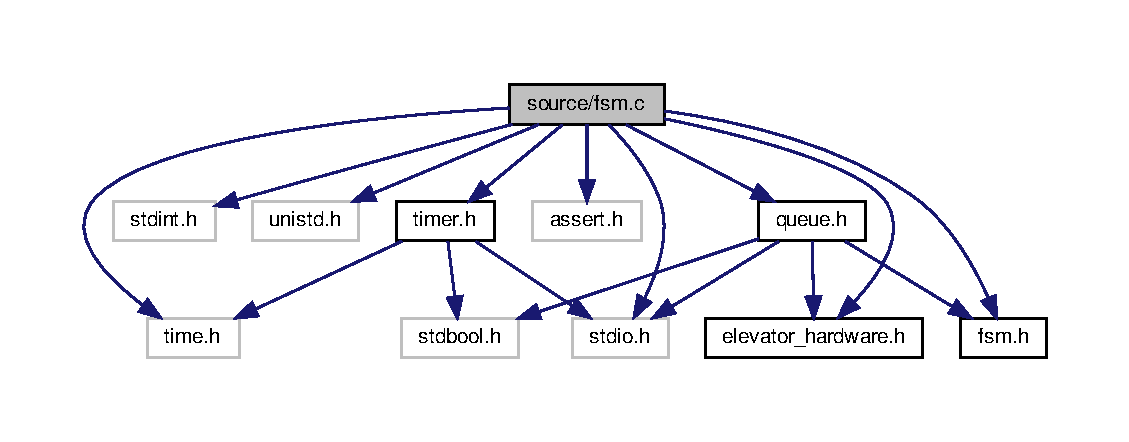
\includegraphics[width=350pt]{fsm_8c__incl}
\end{center}
\end{figure}
\subsection*{Functions}
\begin{DoxyCompactItemize}
\item 
void \hyperlink{fsm_8c_a270932dff1ab343bb350f7c6e02d7a43}{fsm} ()
\begin{DoxyCompactList}\small\item\em The functions main responsibilites is managing the finite state machine. Before entering a switch that manages the state machine it polls\+: \end{DoxyCompactList}\end{DoxyCompactItemize}
\subsection*{Variables}
\begin{DoxyCompactItemize}
\item 
\mbox{\Hypertarget{fsm_8c_a740b52d852a7ed32ae50f2433e7fc8dd}\label{fsm_8c_a740b52d852a7ed32ae50f2433e7fc8dd}} 
static \hyperlink{fsm_8h_a31f24aef3ddd32d2e6538ffff4055d37}{position\+\_\+t} \hyperlink{fsm_8c_a740b52d852a7ed32ae50f2433e7fc8dd}{fsm\+\_\+position} = \hyperlink{fsm_8h_a31f24aef3ddd32d2e6538ffff4055d37a6ce26a62afab55d7606ad4e92428b30c}{U\+N\+K\+N\+O\+WN}
\begin{DoxyCompactList}\small\item\em Local fsm variable used to keep track of the elevators position. \end{DoxyCompactList}\item 
\mbox{\Hypertarget{fsm_8c_ae58b9d6bb7b780f3c1e7fd26baeb5683}\label{fsm_8c_ae58b9d6bb7b780f3c1e7fd26baeb5683}} 
static \hyperlink{fsm_8h_a5b3a976f46b9e6993f1692a09bf2fd60}{floor\+\_\+t} \hyperlink{fsm_8c_ae58b9d6bb7b780f3c1e7fd26baeb5683}{fsm\+\_\+floor} = \hyperlink{fsm_8h_a5b3a976f46b9e6993f1692a09bf2fd60af37d17a566c389570899450d2ccfcd66}{O\+R\+D\+E\+R\+\_\+\+F\+L\+O\+O\+R\+\_\+\+U\+N\+K\+N\+O\+WN}
\begin{DoxyCompactList}\small\item\em Local fsm variable used to keep track of the elevators last or current floor. \end{DoxyCompactList}\item 
\mbox{\Hypertarget{fsm_8c_ae5c3d7b296386537f54acdc123104f68}\label{fsm_8c_ae5c3d7b296386537f54acdc123104f68}} 
static time\+\_\+t \hyperlink{fsm_8c_ae5c3d7b296386537f54acdc123104f68}{fsm\+\_\+timestamp} = 0
\begin{DoxyCompactList}\small\item\em Local fsm variable to keep track of timer responisble for opening the door. \end{DoxyCompactList}\item 
\mbox{\Hypertarget{fsm_8c_a34c0ceaa7f628cf25af6d97bb6775eb4}\label{fsm_8c_a34c0ceaa7f628cf25af6d97bb6775eb4}} 
static \hyperlink{elevator__hardware_8h_ac873de158b370a210216e4b4c7fb218f}{elev\+\_\+motor\+\_\+direction\+\_\+t} \hyperlink{fsm_8c_a34c0ceaa7f628cf25af6d97bb6775eb4}{fsm\+\_\+direction} = \hyperlink{elevator__hardware_8h_ac873de158b370a210216e4b4c7fb218fa92f9028d3af929e10b735b77e0c8de60}{D\+I\+R\+N\+\_\+\+UP}
\begin{DoxyCompactList}\small\item\em Local fsm variable used to keep track of the elevators direction of travel. This can never be D\+I\+R\+N\+\_\+\+S\+T\+OP. \end{DoxyCompactList}\item 
\mbox{\Hypertarget{fsm_8c_a8dedcbff98c01337063f3cc747a20b8d}\label{fsm_8c_a8dedcbff98c01337063f3cc747a20b8d}} 
static \hyperlink{fsm_8h_aa0aafed44fec19806d8f9ad834be1248}{state\+\_\+t} \hyperlink{fsm_8c_a8dedcbff98c01337063f3cc747a20b8d}{fsm\+\_\+state} = \hyperlink{fsm_8h_aa0aafed44fec19806d8f9ad834be1248a0cb1b2c6a7db1f1084886c98909a3f36}{I\+N\+IT}
\begin{DoxyCompactList}\small\item\em Local fsm variable used to keep track of the elevators state. \end{DoxyCompactList}\end{DoxyCompactItemize}


\subsection{Detailed Description}
Implementation of the functions in \hyperlink{fsm_8h}{fsm.\+h}. 



\subsection{Function Documentation}
\mbox{\Hypertarget{fsm_8c_a270932dff1ab343bb350f7c6e02d7a43}\label{fsm_8c_a270932dff1ab343bb350f7c6e02d7a43}} 
\index{fsm.\+c@{fsm.\+c}!fsm@{fsm}}
\index{fsm@{fsm}!fsm.\+c@{fsm.\+c}}
\subsubsection{\texorpdfstring{fsm()}{fsm()}}
{\footnotesize\ttfamily void fsm (\begin{DoxyParamCaption}{ }\end{DoxyParamCaption})}



The functions main responsibilites is managing the finite state machine. Before entering a switch that manages the state machine it polls\+: 


\begin{DoxyItemize}
\item The order buttons
\item floor sensors
\item stop button
\end{DoxyItemize}

The state machine manages the states in the \hyperlink{fsm_8h_aa0aafed44fec19806d8f9ad834be1248}{state\+\_\+t}. The behaviour between the states is described in the state diagram and the sequence diagram.


\begin{DoxyParams}[1]{Parameters}
\mbox{\tt out}  & {\em fsm\+\_\+position} & Elevator position \\
\hline
\mbox{\tt out}  & {\em fsm\+\_\+floor} & Elevator floor \\
\hline
\mbox{\tt out}  & {\em fsm\+\_\+timestamp} & Timestamp \\
\hline
\mbox{\tt out}  & {\em fsm\+\_\+direction} & Elevator direction of travel. This will only ever by D\+I\+R\+N\+\_\+\+UP or D\+I\+R\+N\+\_\+\+D\+O\+WN of \hyperlink{elevator__hardware_8h_ac873de158b370a210216e4b4c7fb218f}{elev\+\_\+motor\+\_\+direction\+\_\+t}. \\
\hline
\mbox{\tt out}  & {\em fsm\+\_\+state} & Elevator state \\
\hline
\end{DoxyParams}


Definition at line 37 of file fsm.\+c.


\hypertarget{fsm_8h}{}\section{source/fsm.h File Reference}
\label{fsm_8h}\index{source/fsm.\+h@{source/fsm.\+h}}


This class that controls the main functions of the elevator. It is responsible for checking input signals in addtion to managing the state of the elevator.  


This graph shows which files directly or indirectly include this file\+:

\hypertarget{main_8c}{}\section{source/main.c File Reference}
\label{main_8c}\index{source/main.\+c@{source/main.\+c}}


The main file of the application.  


{\ttfamily \#include $<$stdio.\+h$>$}\newline
{\ttfamily \#include \char`\"{}elevator\+\_\+hardware.\+h\char`\"{}}\newline
{\ttfamily \#include \char`\"{}fsm.\+h\char`\"{}}\newline
Include dependency graph for main.\+c\+:\nopagebreak
\begin{figure}[H]
\begin{center}
\leavevmode
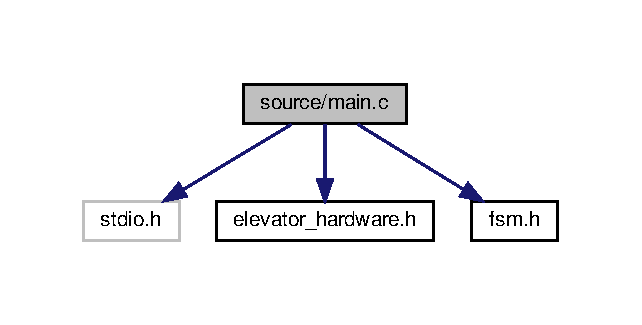
\includegraphics[width=308pt]{main_8c__incl}
\end{center}
\end{figure}


\subsection{Detailed Description}
The main file of the application. 


\hypertarget{queue_8c}{}\section{source/queue.c File Reference}
\label{queue_8c}\index{source/queue.\+c@{source/queue.\+c}}


Implementation of the functions in \hyperlink{queue_8h}{queue.\+h}.  


{\ttfamily \#include $<$stdio.\+h$>$}\newline
{\ttfamily \#include $<$stdint.\+h$>$}\newline
{\ttfamily \#include $<$stdbool.\+h$>$}\newline
{\ttfamily \#include $<$assert.\+h$>$}\newline
{\ttfamily \#include \char`\"{}queue.\+h\char`\"{}}\newline
{\ttfamily \#include \char`\"{}elevator\+\_\+hardware.\+h\char`\"{}}\newline
{\ttfamily \#include \char`\"{}fsm.\+h\char`\"{}}\newline
Include dependency graph for queue.\+c\+:\nopagebreak
\begin{figure}[H]
\begin{center}
\leavevmode
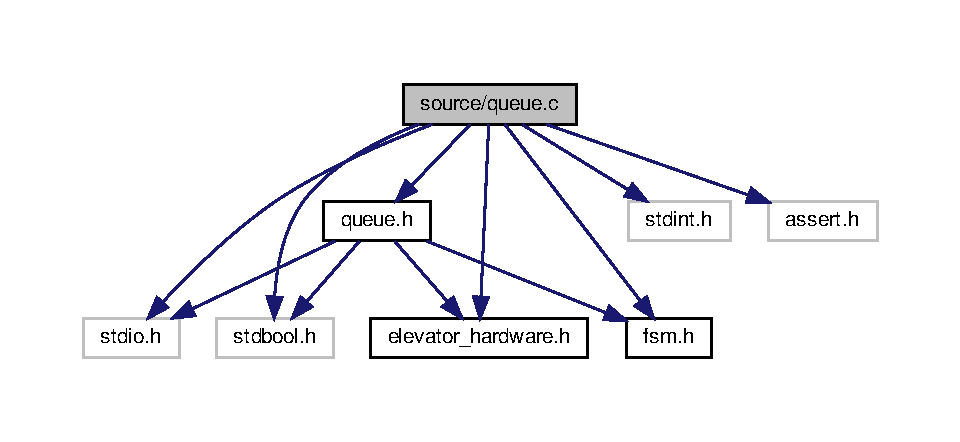
\includegraphics[width=350pt]{queue_8c__incl}
\end{center}
\end{figure}
\subsection*{Functions}
\begin{DoxyCompactItemize}
\item 
void \hyperlink{queue_8c_a600fb7cf1ff3b028fcb97aa1af196065}{queue\+\_\+reset\+\_\+queue} ()
\begin{DoxyCompactList}\small\item\em Deletes all orders in the queue by setting all the order options to the initial value 0. \end{DoxyCompactList}\item 
void \hyperlink{queue_8c_a6b21f1da6ba83e1ee8ac5a64854415b7}{queue\+\_\+delete\+\_\+order} (\hyperlink{fsm_8h_a5b3a976f46b9e6993f1692a09bf2fd60}{floor\+\_\+t} floor)
\begin{DoxyCompactList}\small\item\em Deletes an order in the queue. \end{DoxyCompactList}\item 
void \hyperlink{queue_8c_ad9bbc447a9b368307ff0ea803d6c0fe1}{queue\+\_\+set\+\_\+order} (\hyperlink{elevator__hardware_8h_a5457414cc26332731098d18c37a46e6c}{elev\+\_\+button\+\_\+type\+\_\+t} button, \hyperlink{fsm_8h_a5b3a976f46b9e6993f1692a09bf2fd60}{floor\+\_\+t} floor)
\begin{DoxyCompactList}\small\item\em Sets an order in the queue. \end{DoxyCompactList}\item 
bool \hyperlink{queue_8c_a5f1a2d18955993f8c78589a8ce56dae9}{queue\+\_\+is\+\_\+queue\+\_\+empty} ()
\begin{DoxyCompactList}\small\item\em Checks whether the queue has any orders. \end{DoxyCompactList}\item 
\hyperlink{elevator__hardware_8h_ac873de158b370a210216e4b4c7fb218f}{elev\+\_\+motor\+\_\+direction\+\_\+t} \hyperlink{queue_8c_af2c4aec8d254eec04f73df6b5bba25d4}{queue\+\_\+get\+\_\+next\+\_\+direction} (\hyperlink{fsm_8h_a31f24aef3ddd32d2e6538ffff4055d37}{position\+\_\+t} current\+\_\+position, \hyperlink{elevator__hardware_8h_ac873de158b370a210216e4b4c7fb218f}{elev\+\_\+motor\+\_\+direction\+\_\+t} last\+\_\+direction)
\begin{DoxyCompactList}\small\item\em Checks if the elevator has any orders above, below or at its current position. The function will choose the next direction of the elevator based on these values and will prioritize the orders that is in the direction of the elevator. \end{DoxyCompactList}\item 
bool \hyperlink{queue_8c_a83fd2eb719d7deb1b38cbe8e00603eea}{queue\+\_\+should\+\_\+stop} (\hyperlink{fsm_8h_a31f24aef3ddd32d2e6538ffff4055d37}{position\+\_\+t} \hyperlink{fsm_8c_a740b52d852a7ed32ae50f2433e7fc8dd}{fsm\+\_\+position}, \hyperlink{fsm_8h_a5b3a976f46b9e6993f1692a09bf2fd60}{floor\+\_\+t} \hyperlink{fsm_8c_ae58b9d6bb7b780f3c1e7fd26baeb5683}{fsm\+\_\+floor}, \hyperlink{elevator__hardware_8h_ac873de158b370a210216e4b4c7fb218f}{elev\+\_\+motor\+\_\+direction\+\_\+t} \hyperlink{fsm_8c_a34c0ceaa7f628cf25af6d97bb6775eb4}{fsm\+\_\+direction})
\begin{DoxyCompactList}\small\item\em Checks if the elevator should stop when arriving at a floor, based on orders in the queue array. This function will inform the elevator that it should stop if\+: \end{DoxyCompactList}\end{DoxyCompactItemize}
\subsection*{Variables}
\begin{DoxyCompactItemize}
\item 
\mbox{\Hypertarget{queue_8c_a97dcb6f4deeeacf4e099dd437327b9e7}\label{queue_8c_a97dcb6f4deeeacf4e099dd437327b9e7}} 
static int \hyperlink{queue_8c_a97dcb6f4deeeacf4e099dd437327b9e7}{queue\+\_\+array} \mbox{[}\hyperlink{elevator__hardware_8h_a271dda243b0f5bd7d2053d258eb71962}{N\+\_\+\+B\+U\+T\+T\+O\+NS}\mbox{]}\mbox{[}\hyperlink{elevator__hardware_8h_ae0592e3739e5e1e76234bb1caf9d1305}{N\+\_\+\+F\+L\+O\+O\+RS}\mbox{]}
\begin{DoxyCompactList}\small\item\em A two dimensional array to keep track of the elevators orders. \end{DoxyCompactList}\end{DoxyCompactItemize}


\subsection{Detailed Description}
Implementation of the functions in \hyperlink{queue_8h}{queue.\+h}. 



\subsection{Function Documentation}
\mbox{\Hypertarget{queue_8c_a6b21f1da6ba83e1ee8ac5a64854415b7}\label{queue_8c_a6b21f1da6ba83e1ee8ac5a64854415b7}} 
\index{queue.\+c@{queue.\+c}!queue\+\_\+delete\+\_\+order@{queue\+\_\+delete\+\_\+order}}
\index{queue\+\_\+delete\+\_\+order@{queue\+\_\+delete\+\_\+order}!queue.\+c@{queue.\+c}}
\subsubsection{\texorpdfstring{queue\+\_\+delete\+\_\+order()}{queue\_delete\_order()}}
{\footnotesize\ttfamily void queue\+\_\+delete\+\_\+order (\begin{DoxyParamCaption}\item[{\hyperlink{fsm_8h_a5b3a976f46b9e6993f1692a09bf2fd60}{floor\+\_\+t}}]{floor }\end{DoxyParamCaption})}



Deletes an order in the queue. 


\begin{DoxyParams}[1]{Parameters}
\mbox{\tt in}  & {\em floor} & Floor the elevator is at \\
\hline
\mbox{\tt out}  & {\em queue\+\_\+array} & Queue table \\
\hline
\end{DoxyParams}


Definition at line 35 of file queue.\+c.

Here is the call graph for this function\+:\nopagebreak
\begin{figure}[H]
\begin{center}
\leavevmode
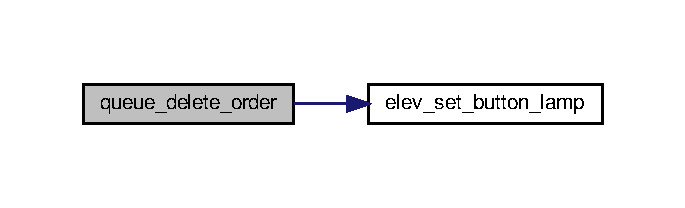
\includegraphics[width=329pt]{queue_8c_a6b21f1da6ba83e1ee8ac5a64854415b7_cgraph}
\end{center}
\end{figure}
\mbox{\Hypertarget{queue_8c_af2c4aec8d254eec04f73df6b5bba25d4}\label{queue_8c_af2c4aec8d254eec04f73df6b5bba25d4}} 
\index{queue.\+c@{queue.\+c}!queue\+\_\+get\+\_\+next\+\_\+direction@{queue\+\_\+get\+\_\+next\+\_\+direction}}
\index{queue\+\_\+get\+\_\+next\+\_\+direction@{queue\+\_\+get\+\_\+next\+\_\+direction}!queue.\+c@{queue.\+c}}
\subsubsection{\texorpdfstring{queue\+\_\+get\+\_\+next\+\_\+direction()}{queue\_get\_next\_direction()}}
{\footnotesize\ttfamily \hyperlink{elevator__hardware_8h_ac873de158b370a210216e4b4c7fb218f}{elev\+\_\+motor\+\_\+direction\+\_\+t} queue\+\_\+get\+\_\+next\+\_\+direction (\begin{DoxyParamCaption}\item[{\hyperlink{fsm_8h_a31f24aef3ddd32d2e6538ffff4055d37}{position\+\_\+t}}]{current\+\_\+position,  }\item[{\hyperlink{elevator__hardware_8h_ac873de158b370a210216e4b4c7fb218f}{elev\+\_\+motor\+\_\+direction\+\_\+t}}]{last\+\_\+direction }\end{DoxyParamCaption})}



Checks if the elevator has any orders above, below or at its current position. The function will choose the next direction of the elevator based on these values and will prioritize the orders that is in the direction of the elevator. 


\begin{DoxyParams}[1]{Parameters}
\mbox{\tt in}  & {\em current\+\_\+position} & The current position of the elevator \\
\hline
\mbox{\tt in}  & {\em last\+\_\+direction} & The direction of travel of the elevator.\\
\hline
\end{DoxyParams}
\begin{DoxyReturn}{Returns}
next direction of the elevator. 
\end{DoxyReturn}


Definition at line 64 of file queue.\+c.

Here is the caller graph for this function\+:\nopagebreak
\begin{figure}[H]
\begin{center}
\leavevmode
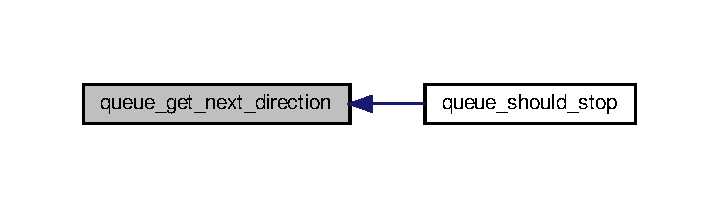
\includegraphics[width=345pt]{queue_8c_af2c4aec8d254eec04f73df6b5bba25d4_icgraph}
\end{center}
\end{figure}
\mbox{\Hypertarget{queue_8c_a5f1a2d18955993f8c78589a8ce56dae9}\label{queue_8c_a5f1a2d18955993f8c78589a8ce56dae9}} 
\index{queue.\+c@{queue.\+c}!queue\+\_\+is\+\_\+queue\+\_\+empty@{queue\+\_\+is\+\_\+queue\+\_\+empty}}
\index{queue\+\_\+is\+\_\+queue\+\_\+empty@{queue\+\_\+is\+\_\+queue\+\_\+empty}!queue.\+c@{queue.\+c}}
\subsubsection{\texorpdfstring{queue\+\_\+is\+\_\+queue\+\_\+empty()}{queue\_is\_queue\_empty()}}
{\footnotesize\ttfamily bool queue\+\_\+is\+\_\+queue\+\_\+empty (\begin{DoxyParamCaption}{ }\end{DoxyParamCaption})}



Checks whether the queue has any orders. 

\begin{DoxyReturn}{Returns}
1 if the queue is empty, 0 if not. 
\end{DoxyReturn}


Definition at line 48 of file queue.\+c.

\mbox{\Hypertarget{queue_8c_a600fb7cf1ff3b028fcb97aa1af196065}\label{queue_8c_a600fb7cf1ff3b028fcb97aa1af196065}} 
\index{queue.\+c@{queue.\+c}!queue\+\_\+reset\+\_\+queue@{queue\+\_\+reset\+\_\+queue}}
\index{queue\+\_\+reset\+\_\+queue@{queue\+\_\+reset\+\_\+queue}!queue.\+c@{queue.\+c}}
\subsubsection{\texorpdfstring{queue\+\_\+reset\+\_\+queue()}{queue\_reset\_queue()}}
{\footnotesize\ttfamily void queue\+\_\+reset\+\_\+queue (\begin{DoxyParamCaption}{ }\end{DoxyParamCaption})}



Deletes all orders in the queue by setting all the order options to the initial value 0. 


\begin{DoxyParams}[1]{Parameters}
\mbox{\tt out}  & {\em queue\+\_\+array} & Queue table \\
\hline
\end{DoxyParams}


Definition at line 24 of file queue.\+c.

Here is the call graph for this function\+:\nopagebreak
\begin{figure}[H]
\begin{center}
\leavevmode
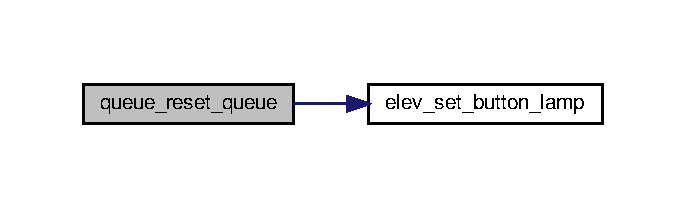
\includegraphics[width=329pt]{queue_8c_a600fb7cf1ff3b028fcb97aa1af196065_cgraph}
\end{center}
\end{figure}
\mbox{\Hypertarget{queue_8c_ad9bbc447a9b368307ff0ea803d6c0fe1}\label{queue_8c_ad9bbc447a9b368307ff0ea803d6c0fe1}} 
\index{queue.\+c@{queue.\+c}!queue\+\_\+set\+\_\+order@{queue\+\_\+set\+\_\+order}}
\index{queue\+\_\+set\+\_\+order@{queue\+\_\+set\+\_\+order}!queue.\+c@{queue.\+c}}
\subsubsection{\texorpdfstring{queue\+\_\+set\+\_\+order()}{queue\_set\_order()}}
{\footnotesize\ttfamily void queue\+\_\+set\+\_\+order (\begin{DoxyParamCaption}\item[{\hyperlink{elevator__hardware_8h_a5457414cc26332731098d18c37a46e6c}{elev\+\_\+button\+\_\+type\+\_\+t}}]{button,  }\item[{\hyperlink{fsm_8h_a5b3a976f46b9e6993f1692a09bf2fd60}{floor\+\_\+t}}]{floor }\end{DoxyParamCaption})}



Sets an order in the queue. 


\begin{DoxyParams}[1]{Parameters}
\mbox{\tt in}  & {\em button} & Hardware buttons \\
\hline
\mbox{\tt in}  & {\em floor} & At a floor \\
\hline
\mbox{\tt out}  & {\em queue\+\_\+array} & Queue table \\
\hline
\end{DoxyParams}


Definition at line 43 of file queue.\+c.

\mbox{\Hypertarget{queue_8c_a83fd2eb719d7deb1b38cbe8e00603eea}\label{queue_8c_a83fd2eb719d7deb1b38cbe8e00603eea}} 
\index{queue.\+c@{queue.\+c}!queue\+\_\+should\+\_\+stop@{queue\+\_\+should\+\_\+stop}}
\index{queue\+\_\+should\+\_\+stop@{queue\+\_\+should\+\_\+stop}!queue.\+c@{queue.\+c}}
\subsubsection{\texorpdfstring{queue\+\_\+should\+\_\+stop()}{queue\_should\_stop()}}
{\footnotesize\ttfamily bool queue\+\_\+should\+\_\+stop (\begin{DoxyParamCaption}\item[{\hyperlink{fsm_8h_a31f24aef3ddd32d2e6538ffff4055d37}{position\+\_\+t}}]{fsm\+\_\+position,  }\item[{\hyperlink{fsm_8h_a5b3a976f46b9e6993f1692a09bf2fd60}{floor\+\_\+t}}]{fsm\+\_\+floor,  }\item[{\hyperlink{elevator__hardware_8h_ac873de158b370a210216e4b4c7fb218f}{elev\+\_\+motor\+\_\+direction\+\_\+t}}]{fsm\+\_\+direction }\end{DoxyParamCaption})}



Checks if the elevator should stop when arriving at a floor, based on orders in the queue array. This function will inform the elevator that it should stop if\+: 


\begin{DoxyItemize}
\item There are no further orders in the direction.
\item There are cab or hall calls in the direction of travel.
\end{DoxyItemize}


\begin{DoxyParams}[1]{Parameters}
\mbox{\tt in}  & {\em fsm\+\_\+position} & The current position of the elevator. \\
\hline
\mbox{\tt in}  & {\em fsm\+\_\+floor} & The current floor of the elevator. \\
\hline
\mbox{\tt in}  & {\em fsm\+\_\+direction} & The direction of travel the elevator.\\
\hline
\end{DoxyParams}
\begin{DoxyReturn}{Returns}
1 of the elevator should stop, 0 if not. 
\end{DoxyReturn}


Definition at line 88 of file queue.\+c.

Here is the call graph for this function\+:\nopagebreak
\begin{figure}[H]
\begin{center}
\leavevmode
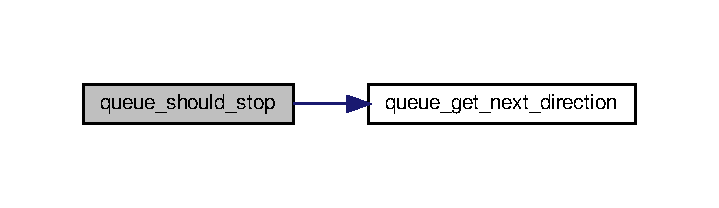
\includegraphics[width=345pt]{queue_8c_a83fd2eb719d7deb1b38cbe8e00603eea_cgraph}
\end{center}
\end{figure}

\hypertarget{queue_8h}{}\section{source/queue.h File Reference}
\label{queue_8h}\index{source/queue.\+h@{source/queue.\+h}}


A queue system that helps the finite state machine (fsm) to carry out the orders received from the elevator hardware.  


{\ttfamily \#include $<$stdio.\+h$>$}\newline
{\ttfamily \#include $<$stdbool.\+h$>$}\newline
{\ttfamily \#include \char`\"{}elevator\+\_\+hardware.\+h\char`\"{}}\newline
{\ttfamily \#include \char`\"{}fsm.\+h\char`\"{}}\newline
Include dependency graph for queue.\+h\+:\nopagebreak
\begin{figure}[H]
\begin{center}
\leavevmode
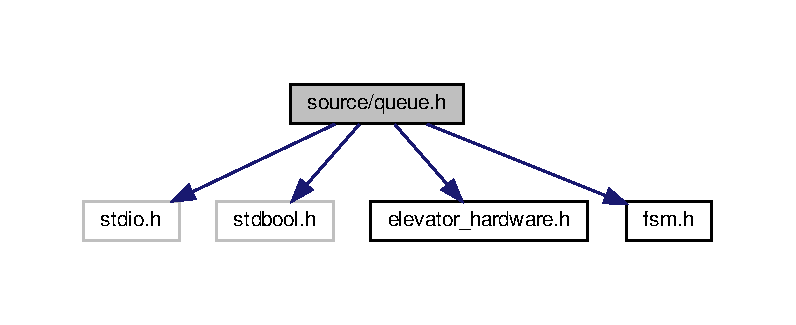
\includegraphics[width=350pt]{queue_8h__incl}
\end{center}
\end{figure}
This graph shows which files directly or indirectly include this file\+:\nopagebreak
\begin{figure}[H]
\begin{center}
\leavevmode
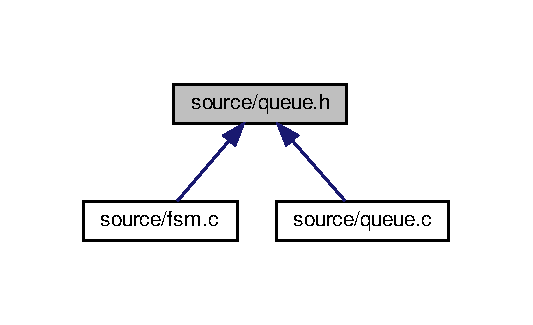
\includegraphics[width=256pt]{queue_8h__dep__incl}
\end{center}
\end{figure}
\subsection*{Functions}
\begin{DoxyCompactItemize}
\item 
void \hyperlink{queue_8h_a600fb7cf1ff3b028fcb97aa1af196065}{queue\+\_\+reset\+\_\+queue} ()
\begin{DoxyCompactList}\small\item\em Deletes all orders in the queue by setting all the order options to the initial value 0. \end{DoxyCompactList}\item 
void \hyperlink{queue_8h_a6b21f1da6ba83e1ee8ac5a64854415b7}{queue\+\_\+delete\+\_\+order} (\hyperlink{fsm_8h_a5b3a976f46b9e6993f1692a09bf2fd60}{floor\+\_\+t} floor)
\begin{DoxyCompactList}\small\item\em Deletes an order in the queue. \end{DoxyCompactList}\item 
void \hyperlink{queue_8h_ad9bbc447a9b368307ff0ea803d6c0fe1}{queue\+\_\+set\+\_\+order} (\hyperlink{elevator__hardware_8h_a5457414cc26332731098d18c37a46e6c}{elev\+\_\+button\+\_\+type\+\_\+t} button, \hyperlink{fsm_8h_a5b3a976f46b9e6993f1692a09bf2fd60}{floor\+\_\+t} floor)
\begin{DoxyCompactList}\small\item\em Sets an order in the queue. \end{DoxyCompactList}\item 
bool \hyperlink{queue_8h_a5f1a2d18955993f8c78589a8ce56dae9}{queue\+\_\+is\+\_\+queue\+\_\+empty} ()
\begin{DoxyCompactList}\small\item\em Checks whether the queue has any orders. \end{DoxyCompactList}\item 
\hyperlink{elevator__hardware_8h_ac873de158b370a210216e4b4c7fb218f}{elev\+\_\+motor\+\_\+direction\+\_\+t} \hyperlink{queue_8h_af2c4aec8d254eec04f73df6b5bba25d4}{queue\+\_\+get\+\_\+next\+\_\+direction} (\hyperlink{fsm_8h_a31f24aef3ddd32d2e6538ffff4055d37}{position\+\_\+t} current\+\_\+position, \hyperlink{elevator__hardware_8h_ac873de158b370a210216e4b4c7fb218f}{elev\+\_\+motor\+\_\+direction\+\_\+t} last\+\_\+direction)
\begin{DoxyCompactList}\small\item\em Checks if the elevator has any orders above, below or at its current position. The function will choose the next direction of the elevator based on these values and will prioritize the orders that is in the direction of the elevator. \end{DoxyCompactList}\item 
bool \hyperlink{queue_8h_a83fd2eb719d7deb1b38cbe8e00603eea}{queue\+\_\+should\+\_\+stop} (\hyperlink{fsm_8h_a31f24aef3ddd32d2e6538ffff4055d37}{position\+\_\+t} \hyperlink{fsm_8c_a740b52d852a7ed32ae50f2433e7fc8dd}{fsm\+\_\+position}, \hyperlink{fsm_8h_a5b3a976f46b9e6993f1692a09bf2fd60}{floor\+\_\+t} \hyperlink{fsm_8c_ae58b9d6bb7b780f3c1e7fd26baeb5683}{fsm\+\_\+floor}, \hyperlink{elevator__hardware_8h_ac873de158b370a210216e4b4c7fb218f}{elev\+\_\+motor\+\_\+direction\+\_\+t} \hyperlink{fsm_8c_a34c0ceaa7f628cf25af6d97bb6775eb4}{fsm\+\_\+direction})
\begin{DoxyCompactList}\small\item\em Checks if the elevator should stop when arriving at a floor, based on orders in the queue array. This function will inform the elevator that it should stop if\+: \end{DoxyCompactList}\end{DoxyCompactItemize}


\subsection{Detailed Description}
A queue system that helps the finite state machine (fsm) to carry out the orders received from the elevator hardware. 



\subsection{Function Documentation}
\mbox{\Hypertarget{queue_8h_a6b21f1da6ba83e1ee8ac5a64854415b7}\label{queue_8h_a6b21f1da6ba83e1ee8ac5a64854415b7}} 
\index{queue.\+h@{queue.\+h}!queue\+\_\+delete\+\_\+order@{queue\+\_\+delete\+\_\+order}}
\index{queue\+\_\+delete\+\_\+order@{queue\+\_\+delete\+\_\+order}!queue.\+h@{queue.\+h}}
\subsubsection{\texorpdfstring{queue\+\_\+delete\+\_\+order()}{queue\_delete\_order()}}
{\footnotesize\ttfamily void queue\+\_\+delete\+\_\+order (\begin{DoxyParamCaption}\item[{\hyperlink{fsm_8h_a5b3a976f46b9e6993f1692a09bf2fd60}{floor\+\_\+t}}]{floor }\end{DoxyParamCaption})}



Deletes an order in the queue. 


\begin{DoxyParams}[1]{Parameters}
\mbox{\tt in}  & {\em floor} & Floor the elevator is at \\
\hline
\mbox{\tt out}  & {\em queue\+\_\+array} & Queue table \\
\hline
\end{DoxyParams}


Definition at line 35 of file queue.\+c.

Here is the call graph for this function\+:\nopagebreak
\begin{figure}[H]
\begin{center}
\leavevmode
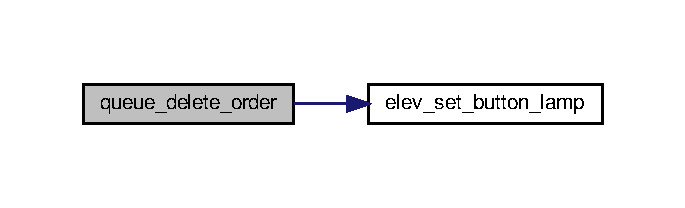
\includegraphics[width=329pt]{queue_8h_a6b21f1da6ba83e1ee8ac5a64854415b7_cgraph}
\end{center}
\end{figure}
\mbox{\Hypertarget{queue_8h_af2c4aec8d254eec04f73df6b5bba25d4}\label{queue_8h_af2c4aec8d254eec04f73df6b5bba25d4}} 
\index{queue.\+h@{queue.\+h}!queue\+\_\+get\+\_\+next\+\_\+direction@{queue\+\_\+get\+\_\+next\+\_\+direction}}
\index{queue\+\_\+get\+\_\+next\+\_\+direction@{queue\+\_\+get\+\_\+next\+\_\+direction}!queue.\+h@{queue.\+h}}
\subsubsection{\texorpdfstring{queue\+\_\+get\+\_\+next\+\_\+direction()}{queue\_get\_next\_direction()}}
{\footnotesize\ttfamily \hyperlink{elevator__hardware_8h_ac873de158b370a210216e4b4c7fb218f}{elev\+\_\+motor\+\_\+direction\+\_\+t} queue\+\_\+get\+\_\+next\+\_\+direction (\begin{DoxyParamCaption}\item[{\hyperlink{fsm_8h_a31f24aef3ddd32d2e6538ffff4055d37}{position\+\_\+t}}]{current\+\_\+position,  }\item[{\hyperlink{elevator__hardware_8h_ac873de158b370a210216e4b4c7fb218f}{elev\+\_\+motor\+\_\+direction\+\_\+t}}]{last\+\_\+direction }\end{DoxyParamCaption})}



Checks if the elevator has any orders above, below or at its current position. The function will choose the next direction of the elevator based on these values and will prioritize the orders that is in the direction of the elevator. 


\begin{DoxyParams}[1]{Parameters}
\mbox{\tt in}  & {\em current\+\_\+position} & The current position of the elevator \\
\hline
\mbox{\tt in}  & {\em last\+\_\+direction} & The direction of travel of the elevator.\\
\hline
\end{DoxyParams}
\begin{DoxyReturn}{Returns}
next direction of the elevator. 
\end{DoxyReturn}


Definition at line 64 of file queue.\+c.

Here is the caller graph for this function\+:\nopagebreak
\begin{figure}[H]
\begin{center}
\leavevmode
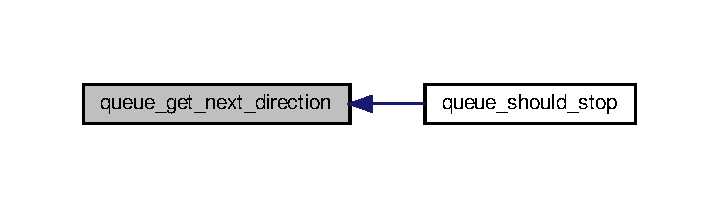
\includegraphics[width=345pt]{queue_8h_af2c4aec8d254eec04f73df6b5bba25d4_icgraph}
\end{center}
\end{figure}
\mbox{\Hypertarget{queue_8h_a5f1a2d18955993f8c78589a8ce56dae9}\label{queue_8h_a5f1a2d18955993f8c78589a8ce56dae9}} 
\index{queue.\+h@{queue.\+h}!queue\+\_\+is\+\_\+queue\+\_\+empty@{queue\+\_\+is\+\_\+queue\+\_\+empty}}
\index{queue\+\_\+is\+\_\+queue\+\_\+empty@{queue\+\_\+is\+\_\+queue\+\_\+empty}!queue.\+h@{queue.\+h}}
\subsubsection{\texorpdfstring{queue\+\_\+is\+\_\+queue\+\_\+empty()}{queue\_is\_queue\_empty()}}
{\footnotesize\ttfamily bool queue\+\_\+is\+\_\+queue\+\_\+empty (\begin{DoxyParamCaption}{ }\end{DoxyParamCaption})}



Checks whether the queue has any orders. 

\begin{DoxyReturn}{Returns}
1 if the queue is empty, 0 if not. 
\end{DoxyReturn}


Definition at line 48 of file queue.\+c.

\mbox{\Hypertarget{queue_8h_a600fb7cf1ff3b028fcb97aa1af196065}\label{queue_8h_a600fb7cf1ff3b028fcb97aa1af196065}} 
\index{queue.\+h@{queue.\+h}!queue\+\_\+reset\+\_\+queue@{queue\+\_\+reset\+\_\+queue}}
\index{queue\+\_\+reset\+\_\+queue@{queue\+\_\+reset\+\_\+queue}!queue.\+h@{queue.\+h}}
\subsubsection{\texorpdfstring{queue\+\_\+reset\+\_\+queue()}{queue\_reset\_queue()}}
{\footnotesize\ttfamily void queue\+\_\+reset\+\_\+queue (\begin{DoxyParamCaption}{ }\end{DoxyParamCaption})}



Deletes all orders in the queue by setting all the order options to the initial value 0. 


\begin{DoxyParams}[1]{Parameters}
\mbox{\tt out}  & {\em queue\+\_\+array} & Queue table \\
\hline
\end{DoxyParams}


Definition at line 24 of file queue.\+c.

Here is the call graph for this function\+:\nopagebreak
\begin{figure}[H]
\begin{center}
\leavevmode
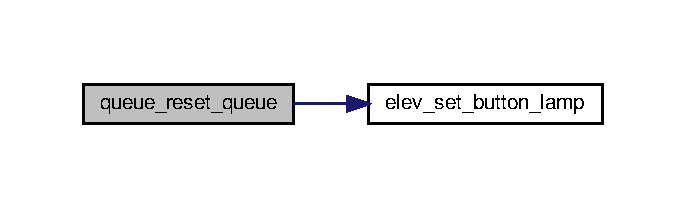
\includegraphics[width=329pt]{queue_8h_a600fb7cf1ff3b028fcb97aa1af196065_cgraph}
\end{center}
\end{figure}
\mbox{\Hypertarget{queue_8h_ad9bbc447a9b368307ff0ea803d6c0fe1}\label{queue_8h_ad9bbc447a9b368307ff0ea803d6c0fe1}} 
\index{queue.\+h@{queue.\+h}!queue\+\_\+set\+\_\+order@{queue\+\_\+set\+\_\+order}}
\index{queue\+\_\+set\+\_\+order@{queue\+\_\+set\+\_\+order}!queue.\+h@{queue.\+h}}
\subsubsection{\texorpdfstring{queue\+\_\+set\+\_\+order()}{queue\_set\_order()}}
{\footnotesize\ttfamily void queue\+\_\+set\+\_\+order (\begin{DoxyParamCaption}\item[{\hyperlink{elevator__hardware_8h_a5457414cc26332731098d18c37a46e6c}{elev\+\_\+button\+\_\+type\+\_\+t}}]{button,  }\item[{\hyperlink{fsm_8h_a5b3a976f46b9e6993f1692a09bf2fd60}{floor\+\_\+t}}]{floor }\end{DoxyParamCaption})}



Sets an order in the queue. 


\begin{DoxyParams}[1]{Parameters}
\mbox{\tt in}  & {\em button} & Hardware buttons \\
\hline
\mbox{\tt in}  & {\em floor} & At a floor \\
\hline
\mbox{\tt out}  & {\em queue\+\_\+array} & Queue table \\
\hline
\end{DoxyParams}


Definition at line 43 of file queue.\+c.

\mbox{\Hypertarget{queue_8h_a83fd2eb719d7deb1b38cbe8e00603eea}\label{queue_8h_a83fd2eb719d7deb1b38cbe8e00603eea}} 
\index{queue.\+h@{queue.\+h}!queue\+\_\+should\+\_\+stop@{queue\+\_\+should\+\_\+stop}}
\index{queue\+\_\+should\+\_\+stop@{queue\+\_\+should\+\_\+stop}!queue.\+h@{queue.\+h}}
\subsubsection{\texorpdfstring{queue\+\_\+should\+\_\+stop()}{queue\_should\_stop()}}
{\footnotesize\ttfamily bool queue\+\_\+should\+\_\+stop (\begin{DoxyParamCaption}\item[{\hyperlink{fsm_8h_a31f24aef3ddd32d2e6538ffff4055d37}{position\+\_\+t}}]{fsm\+\_\+position,  }\item[{\hyperlink{fsm_8h_a5b3a976f46b9e6993f1692a09bf2fd60}{floor\+\_\+t}}]{fsm\+\_\+floor,  }\item[{\hyperlink{elevator__hardware_8h_ac873de158b370a210216e4b4c7fb218f}{elev\+\_\+motor\+\_\+direction\+\_\+t}}]{fsm\+\_\+direction }\end{DoxyParamCaption})}



Checks if the elevator should stop when arriving at a floor, based on orders in the queue array. This function will inform the elevator that it should stop if\+: 


\begin{DoxyItemize}
\item There are no further orders in the direction.
\item There are cab or hall calls in the direction of travel.
\end{DoxyItemize}


\begin{DoxyParams}[1]{Parameters}
\mbox{\tt in}  & {\em fsm\+\_\+position} & The current position of the elevator. \\
\hline
\mbox{\tt in}  & {\em fsm\+\_\+floor} & The current floor of the elevator. \\
\hline
\mbox{\tt in}  & {\em fsm\+\_\+direction} & The direction of travel the elevator.\\
\hline
\end{DoxyParams}
\begin{DoxyReturn}{Returns}
1 of the elevator should stop, 0 if not. 
\end{DoxyReturn}


Definition at line 88 of file queue.\+c.

Here is the call graph for this function\+:\nopagebreak
\begin{figure}[H]
\begin{center}
\leavevmode
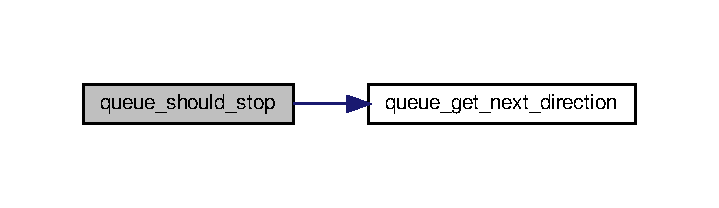
\includegraphics[width=345pt]{queue_8h_a83fd2eb719d7deb1b38cbe8e00603eea_cgraph}
\end{center}
\end{figure}

\hypertarget{timer_8c}{}\section{source/timer.c File Reference}
\label{timer_8c}\index{source/timer.\+c@{source/timer.\+c}}


Implementation of the functions in \hyperlink{timer_8h}{timer.\+h}.  


{\ttfamily \#include $<$stdio.\+h$>$}\newline
{\ttfamily \#include $<$stdbool.\+h$>$}\newline
{\ttfamily \#include $<$time.\+h$>$}\newline
{\ttfamily \#include \char`\"{}timer.\+h\char`\"{}}\newline
Include dependency graph for timer.\+c\+:\nopagebreak
\begin{figure}[H]
\begin{center}
\leavevmode
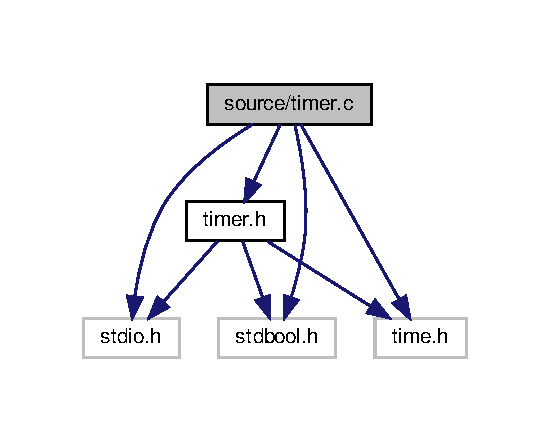
\includegraphics[width=264pt]{timer_8c__incl}
\end{center}
\end{figure}
\subsection*{Functions}
\begin{DoxyCompactItemize}
\item 
time\+\_\+t \hyperlink{timer_8c_a4f7af40cfc5b42ea4f3ecd8e733a5bbf}{timer\+\_\+start\+\_\+timer} ()
\begin{DoxyCompactList}\small\item\em Starts a fictious timer by returning timestamp of the current time of the system. \end{DoxyCompactList}\item 
bool \hyperlink{timer_8c_a01822a31178b24ba570dd599a4549432}{timer\+\_\+is\+\_\+timer\+\_\+expired} (time\+\_\+t start\+\_\+timestamp)
\begin{DoxyCompactList}\small\item\em Check whether 3 seconds have passed since the timer started. \end{DoxyCompactList}\end{DoxyCompactItemize}


\subsection{Detailed Description}
Implementation of the functions in \hyperlink{timer_8h}{timer.\+h}. 



\subsection{Function Documentation}
\mbox{\Hypertarget{timer_8c_a01822a31178b24ba570dd599a4549432}\label{timer_8c_a01822a31178b24ba570dd599a4549432}} 
\index{timer.\+c@{timer.\+c}!timer\+\_\+is\+\_\+timer\+\_\+expired@{timer\+\_\+is\+\_\+timer\+\_\+expired}}
\index{timer\+\_\+is\+\_\+timer\+\_\+expired@{timer\+\_\+is\+\_\+timer\+\_\+expired}!timer.\+c@{timer.\+c}}
\subsubsection{\texorpdfstring{timer\+\_\+is\+\_\+timer\+\_\+expired()}{timer\_is\_timer\_expired()}}
{\footnotesize\ttfamily bool timer\+\_\+is\+\_\+timer\+\_\+expired (\begin{DoxyParamCaption}\item[{time\+\_\+t}]{start\+\_\+timestamp }\end{DoxyParamCaption})}



Check whether 3 seconds have passed since the timer started. 


\begin{DoxyParams}[1]{Parameters}
\mbox{\tt in}  & {\em start\+\_\+time} & Start time of timer.\\
\hline
\end{DoxyParams}
\begin{DoxyReturn}{Returns}
1 if the timer is expired, 0 if not. 
\end{DoxyReturn}


Definition at line 17 of file timer.\+c.

\mbox{\Hypertarget{timer_8c_a4f7af40cfc5b42ea4f3ecd8e733a5bbf}\label{timer_8c_a4f7af40cfc5b42ea4f3ecd8e733a5bbf}} 
\index{timer.\+c@{timer.\+c}!timer\+\_\+start\+\_\+timer@{timer\+\_\+start\+\_\+timer}}
\index{timer\+\_\+start\+\_\+timer@{timer\+\_\+start\+\_\+timer}!timer.\+c@{timer.\+c}}
\subsubsection{\texorpdfstring{timer\+\_\+start\+\_\+timer()}{timer\_start\_timer()}}
{\footnotesize\ttfamily time\+\_\+t timer\+\_\+start\+\_\+timer (\begin{DoxyParamCaption}{ }\end{DoxyParamCaption})}



Starts a fictious timer by returning timestamp of the current time of the system. 

\begin{DoxyReturn}{Returns}
the start time. 
\end{DoxyReturn}


Definition at line 12 of file timer.\+c.


\hypertarget{timer_8h}{}\section{source/timer.h File Reference}
\label{timer_8h}\index{source/timer.\+h@{source/timer.\+h}}


A smaller module that manages the time dependent operations of the state machine.  


{\ttfamily \#include $<$stdio.\+h$>$}\newline
{\ttfamily \#include $<$stdbool.\+h$>$}\newline
{\ttfamily \#include $<$time.\+h$>$}\newline
Include dependency graph for timer.\+h\+:\nopagebreak
\begin{figure}[H]
\begin{center}
\leavevmode
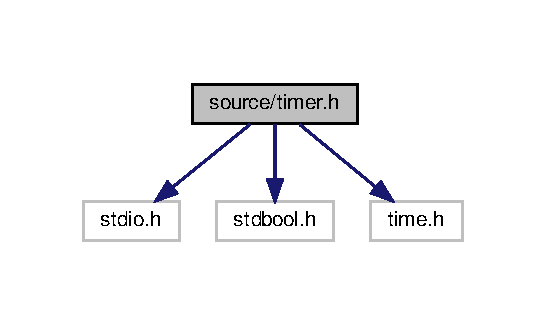
\includegraphics[width=262pt]{timer_8h__incl}
\end{center}
\end{figure}
This graph shows which files directly or indirectly include this file\+:\nopagebreak
\begin{figure}[H]
\begin{center}
\leavevmode
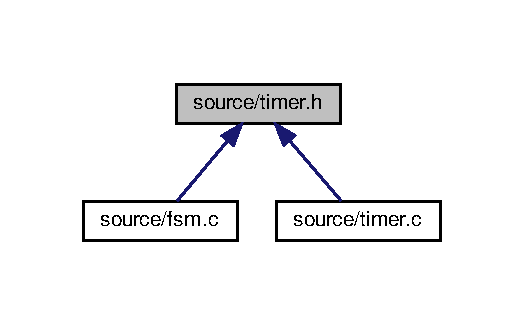
\includegraphics[width=252pt]{timer_8h__dep__incl}
\end{center}
\end{figure}
\subsection*{Functions}
\begin{DoxyCompactItemize}
\item 
time\+\_\+t \hyperlink{timer_8h_a4f7af40cfc5b42ea4f3ecd8e733a5bbf}{timer\+\_\+start\+\_\+timer} ()
\begin{DoxyCompactList}\small\item\em Starts a fictious timer by returning timestamp of the current time of the system. \end{DoxyCompactList}\item 
bool \hyperlink{timer_8h_a01822a31178b24ba570dd599a4549432}{timer\+\_\+is\+\_\+timer\+\_\+expired} (time\+\_\+t start\+\_\+timestamp)
\begin{DoxyCompactList}\small\item\em Check whether 3 seconds have passed since the timer started. \end{DoxyCompactList}\end{DoxyCompactItemize}


\subsection{Detailed Description}
A smaller module that manages the time dependent operations of the state machine. 



\subsection{Function Documentation}
\mbox{\Hypertarget{timer_8h_a01822a31178b24ba570dd599a4549432}\label{timer_8h_a01822a31178b24ba570dd599a4549432}} 
\index{timer.\+h@{timer.\+h}!timer\+\_\+is\+\_\+timer\+\_\+expired@{timer\+\_\+is\+\_\+timer\+\_\+expired}}
\index{timer\+\_\+is\+\_\+timer\+\_\+expired@{timer\+\_\+is\+\_\+timer\+\_\+expired}!timer.\+h@{timer.\+h}}
\subsubsection{\texorpdfstring{timer\+\_\+is\+\_\+timer\+\_\+expired()}{timer\_is\_timer\_expired()}}
{\footnotesize\ttfamily bool timer\+\_\+is\+\_\+timer\+\_\+expired (\begin{DoxyParamCaption}\item[{time\+\_\+t}]{start\+\_\+timestamp }\end{DoxyParamCaption})}



Check whether 3 seconds have passed since the timer started. 


\begin{DoxyParams}[1]{Parameters}
\mbox{\tt in}  & {\em start\+\_\+time} & Start time of timer.\\
\hline
\end{DoxyParams}
\begin{DoxyReturn}{Returns}
1 if the timer is expired, 0 if not. 
\end{DoxyReturn}


Definition at line 17 of file timer.\+c.

\mbox{\Hypertarget{timer_8h_a4f7af40cfc5b42ea4f3ecd8e733a5bbf}\label{timer_8h_a4f7af40cfc5b42ea4f3ecd8e733a5bbf}} 
\index{timer.\+h@{timer.\+h}!timer\+\_\+start\+\_\+timer@{timer\+\_\+start\+\_\+timer}}
\index{timer\+\_\+start\+\_\+timer@{timer\+\_\+start\+\_\+timer}!timer.\+h@{timer.\+h}}
\subsubsection{\texorpdfstring{timer\+\_\+start\+\_\+timer()}{timer\_start\_timer()}}
{\footnotesize\ttfamily time\+\_\+t timer\+\_\+start\+\_\+timer (\begin{DoxyParamCaption}{ }\end{DoxyParamCaption})}



Starts a fictious timer by returning timestamp of the current time of the system. 

\begin{DoxyReturn}{Returns}
the start time. 
\end{DoxyReturn}


Definition at line 12 of file timer.\+c.


%--- End generated contents ---

% Index
\backmatter
\newpage
\phantomsection
\clearemptydoublepage
\addcontentsline{toc}{chapter}{Index}
\printindex

\end{document}
